\section{Versionshistorie}

\begin{table}[h]
\begin{tabularx}{\textwidth}{|l|X|l|l|}
\hline
\thead{Version} & \thead{Änderung} & \thead{Bearbeiter} & \thead{Datum} \\	\hline
v1.0 & Erstellung des Dokumentes, Erarbeiten der Kapitel \nameref{Vorwort}, \nameref{Vorbereitung} und \nameref{Zeitplan} & Damian Moser & \DTMdisplaydate{2018}{05}{22}{-1} \\	\hline
V1.1 & Erarbeiten der Kapitel \nameref{Arbeitsmethodik}, \nameref{Aufgabenstellung}, \nameref{Testen Theorie} und \nameref{Testen in der Abacus} & Damian Moser & \DTMdisplaydate{2018}{05}{28}{-1} \\    \hline
v1.2 & Erarbeiten der Kapitel \nameref{goodvsbad} und \nameref{Datenspeicherung}, erweitern des Kapitels \nameref{Testen in der Abacus} & Damian Moser & \DTMdisplaydate{2018}{05}{29}{-1} \\ \hline
v1.3 & Erarbeiten der Kapitel \nameref{Testmöglichkeiten}, erweitern des Kapitels \nameref{Datenspeicherung} & Damian Moser & \DTMdisplaydate{2018}{06}{01}{-1} \\ \hline
v1.4 & Erarbeiten des Kapitels \nameref{Testmethoden2}, erweitern des Kapitels \nameref{Offene Fragen} & Damian Moser & \DTMdisplaydate{2018}{06}{04}{-1} \\ \hline
v1.5 & Erstellen des Kapitels \nameref{Auswertung} & Damian Moser & \DTMdisplaydate{2018}{06}{05}{-1} \\ \hline
v1.6 & Erweitern des Kapitels \nameref{Auswertung} & Damian Moser & \DTMdisplaydate{2018}{06}{08}{-1} \\ \hline
v1.7 & Erweitern des Kapitels \nameref{Auswertung} & Damian Moser & \DTMdisplaydate{2018}{06}{11}{-1} \\ \hline
v1.8 & Erarbeiten des Kapitels \nameref{eigene Testmethode}, erweitern des Kapitels \nameref{Auswertung} & Damian Moser & \DTMdisplaydate{2018}{06}{12}{-1} \\ \hline
v1.9 & Erweitern des Kapitels \nameref{eigene Testmethode} & Damian Moser & \DTMdisplaydate{2018}{06}{14}{-1} \\ \hline
v1.10 & Erarbeiten des Kapitels \nameref{Migrationskonzept} & Damian Moser & \DTMdisplaydate{2018}{06}{15}{-1} \\ \hline
v1.11 & Erarbeiten des Kapitels \nameref{Fazit} & Damian Moser & \DTMdisplaydate{2018}{06}{18}{-1} \\ \hline
v1.12 & Erweitern des Kapitels \nameref{Fazit} & Damian Moser & \DTMdisplaydate{2018}{06}{19}{-1} \\ \hline
v2.0 & Dokument auf letzten sauberen Stand bringen & Damian Moser & \DTMdisplaydate{2018}{06}{19}{-1} \\ \hline
\end{tabularx}
\caption{Versionsübersicht}
\end{table}

\section{Vorwort} \label{Vorwort}
Nach der Bildungsverordnung (BiVo 2014), muss ein Informatiker-Lehrling im zweiten Semester des vierten Lehrjahrs eine \enquote{Individuelle Projektarbeit}, kurz IPA, ablegen. Dabei handelt es sich um eine Aufgabe, welche vom Lehrbetrieb gestellt wird und innert 120 Stunden geplant, entwickelt und abgeschlossen werden muss. Die gestellte Aufgabe beinhaltet die Evaluation und Analyse von \enquote{Test-Methodiken} in der Abacus.\\
Diese Dokumentation ist ein Teil dieser IPA und zeigt mein Vorgehen bei dieser Arbeit auf. Es wird auf verschiedene Aspekte der Planung und Realisierung eingegangen und verschiedene Aspekte erläutert.

\section{Vorbereitung} \label{Vorbereitung}

\subsection{Werkzeuge}
\begin{table}[H]
\begin{tabularx}{\textwidth}{|l|l|X|}
\hline
\thead{Programmname} & \thead{Kategorie} & \thead{Verwendungszweck} \\	\hline
Texmaker & Textbearbeitung für \LaTeX & Schreiben der Dokumentation in \LaTeX \\	\hline
MiKTeX & \LaTeX-Interpreter & Erstellen des PDFs aus den in \LaTeX\ geschriebenen Dokumenten \\    \hline
Excel & Tabellenkalkulation & Erstellen und Auswerten der Zeitplanung \\    \hline
Notepad++ & Texteditor & Anschauen und Bearbeiten verschiedener Dateitypen \\    \hline
InteliJ IDEA & \ac{IDE} & Entwicklungsumgebung für Javacode \\    \hline
Abacus & ERP-Software & Stellt die Voraussetzungen der Datenstruktur und Grundlagen der Tests \\    \hline
JDBX & Datenbankeditor & Anzeigen, bearbeiten von Daten in der Datenbank \\    \hline
Firefox & Internetbrowser & Für die Informationsbeschaffung im Internet\\ \hline
Diktiergerät & Audio-Aufnahme & App auf dem Smartphone für Audioaufnahmen \\ \hline
\end{tabularx}
\caption{Verwendete Werkzeuge}
\end{table}
\subsection{Datensicherungskonzept}
Damit ich meine Arbeit nicht einfach verlieren kann, brauche ich ein robustes Backup-Konzept. Deshalb werden die Dokumente täglich auf einem Datenspeicherserver gespeichert. Dies habe ich mit folgendem Skript realisiert.
\begin{lstlisting}[language=bash]
robocopy .\2018 \\abadata02\exchange\moserd\ipaupdate /E
\end{lstlisting}
Dies wird jeweils einmal am Tag von der Aufgabenplanung gestartet. So kann ich maximal Arbeit von einem Tag verlieren. Auf der anderen Seite habe ich den Sourcecode, welchen ich schreiben werde. Dieser wird, sobald der Stand stabil ist, auf den Subversion-Server geladen. Um die Zwischenstände zu sichern, werde ich bei Bedarf einen Patch generieren und diesen ebenfalls auf dem Datenspeicherserver sichern.

\section{Arbeitsmethodik} \label{Arbeitsmethodik}
In der Schule haben wir einige Arbeitsmethoden durchgenommen. Dabei hat jede Methodik ihre eigenen Vor- und Nachteile. Diese gilt es abzuwägen. 
\subsection{Wasserfallmodell}
Das Wasserfallmodell ist ein lineares Modell. Es wird primär in der Softwareentwicklung eingesetzt. Dabei wird das Projekt in verschiedene Phasen abgetrennt. Diese werden jeweils abgetrennt ausgeführt und überlappen sich nicht. Nach jeder Phase hat mein ein neues Produkt (Entweder ein Dokument oder ein lauffähiges Produkt).
\begin{figure}[H]
	\centering
	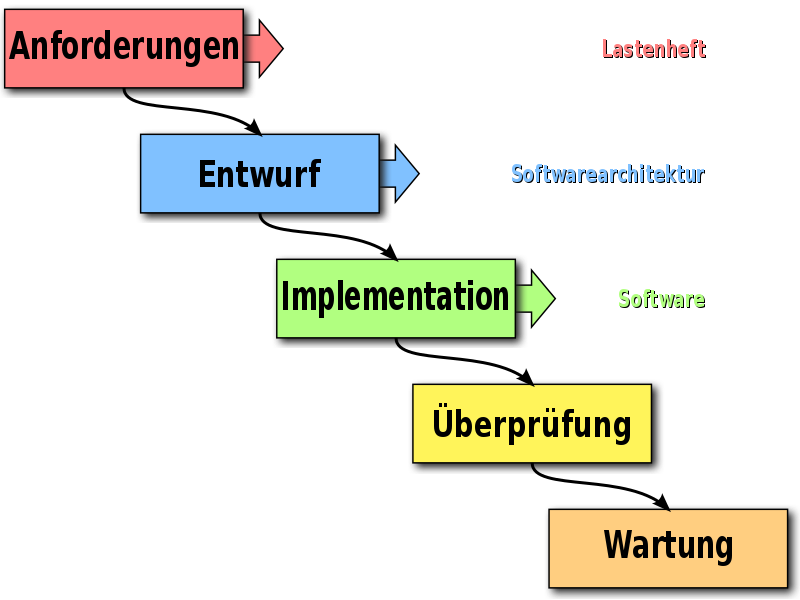
\includegraphics[width=0.6\textwidth]{wasserfallmodell}
	\caption{Wasserfallmodell, \cite{wiki:Wasserfallmodellimage}}
\end{figure}
\subsubsection{Pro}
\begin{itemize}
\item Jede Phase hat ein klar definiertes Resultat, welches sich einfach überprüfen lässt.
\end{itemize}
\subsubsection{Contra}
\begin{itemize}
\item Aufgaben können nicht parallel ausgeführt werden, Phasen können sich nicht überschneiden.
\item Fehler in der Planung lassen sich erst spät erkennen.
\item Bei einer falschen Planung kann ein Projekt schnell ausarten. \cite{wiki:Wasserfallmodell}
\end{itemize}
\subsection{IPERKA}
IPERKA steht für Informieren, Planen, Entscheiden, Realisieren, Kontrollieren und Auswerten. Dies sind die Schritte, welche nacheinander ausgeführt werden. Diese Schritte werden klar voneinander abgegrenzt. Der Schwerpunkt liegt hier vor allem auf der Planung, da häufig schon zu früh mit der Realisierung begonnen wird.
\begin{figure}[H]
	\centering
	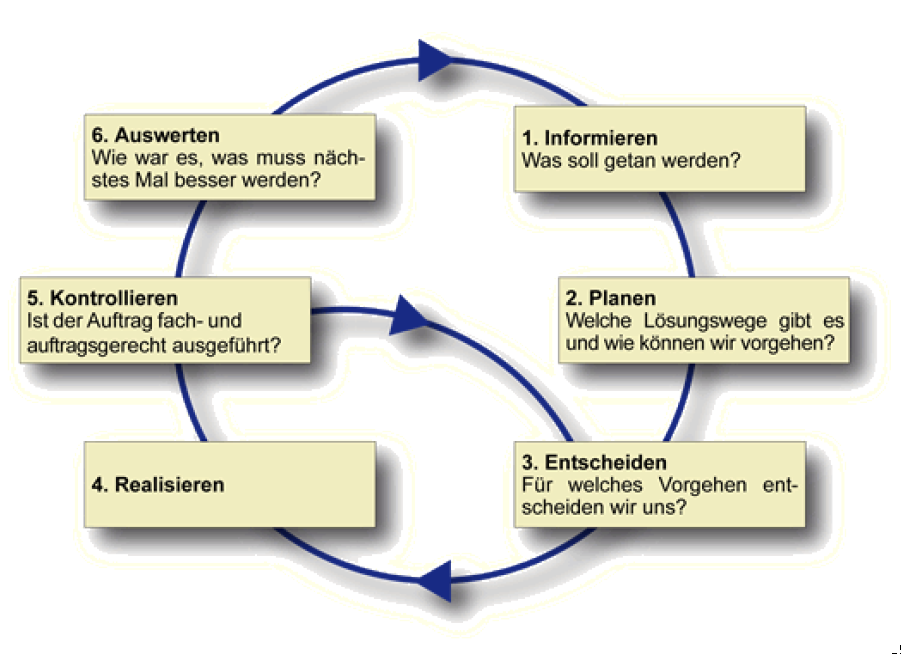
\includegraphics[width=0.7\textwidth]{iperka}
	\caption{IPERKA-Modell, \cite{web:iperkaimage}}
\end{figure}
\subsubsection{Pro}
\begin{itemize}
\item Arbeitsschritte lassen sich einfach den einzelnen Phasen zuordnen.
\item Geringer Administrativer Aufwand.
\item Selber schon positive Erfahrungen damit gemacht.
\item Besonders geeignet für kleine Projekte
\end{itemize}
\subsubsection{Contra}
\begin{itemize}
\item Aufgaben können nicht parallel ausgeführt werden, Phasen können sich nicht überschneiden. \cite{web:iperka}
\end{itemize}
\subsection{Scrum}
Scrum ist eine iterative Methode, welche für Teams besonders geeignet ist. Einzelne Tasks werden gesammelt und im Produkt-Backlog gehalten. Der Scrummaster entscheidet dann, welche Tasks als nächstes realisiert werden soll. Dafür wird ein Sprint erstellt. Dieser Sprint beinhaltet einen abgegrenzten Zeitraum und den Sprint-Backlog mit der Arbeit, welche als nächstes erledigt werden muss. Nach dem Sprint hat man wieder ein Produkt, welches ausgeliefert werden könnte. Auch hat man nach dem Sprint die Möglichkeit, die getane Arbeit zu realisieren und Änderungen in der Planung zu machen.
\begin{figure}[H]
	\centering
	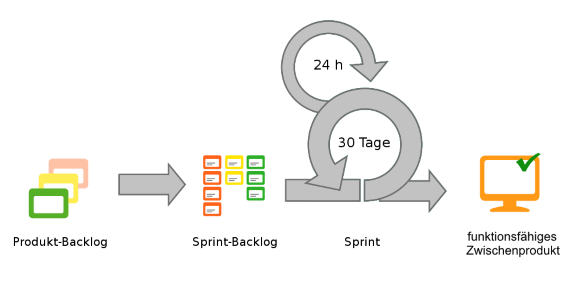
\includegraphics[width=0.8\textwidth]{scrum}
	\caption{Scrum-Modell, \cite{web:scrumimage}}
\end{figure}
\subsubsection{Pro}
\begin{itemize}
\item Die Planung lässt sich jederzeit wieder anpassen
\item Man erhält schnell Anfangsprodukt
\end{itemize}
\subsubsection{Contra}
\begin{itemize}
\item Da ein Sprint selber mehrere Wochen dauert, eher ungeeignet für die IPA.
\item Optimal für Teams.
\end{itemize}

\subsection{Evaluation}
Um dieses Projekt zu realisieren, ist von den aufgelisteten Methoden IPERKA das geeignetste. Da aber auch diese Nachteile hat, auf welche ich gerne verzichten würde, werde ich es ein wenig anders umsetzten. Die ganze IPA werde ich mit IPERKA umsetzten. Aber der Punkt realisieren wird ein wenig abgeändert. Die einzelnen Testmethoden werde ich nacheinander abarbeiten, anstatt alle gleichzeitig. So werden die Testmethoden wie als kleine Sub-IPERKA-Projekte gehandhabt. So kombiniere ich das Beste aus IPERKA und Scrum.
\begin{table}[H]
\begin{tabularx}{\textwidth}{|l|l|X|}
\hline
\thead{Prozessschritt IPA} & \thead{Prozessschritt Subprozess} & \thead{Aufgabe} \\	\hline
\multicolumn{3}{|c|}{[...]} \\ \hline
Informieren & & Offene Fragen klären\\	\hline
\multicolumn{3}{|c|}{[...]} \\ \hline
Planen & & Erstellen einer Bewertungsmatrix\\	\hline
Planen & & Konzept für Messung der Kriterien \\    \hline
\multicolumn{3}{|c|}{[...]} \\ \hline
\multicolumn{3}{|c|}{\textbf{Start erster Subprozess}} \\ \hline
Realisieren & Informieren, Planen, Entscheiden & Analyse Testmöglichkeit 1 \\ \hline
Realisieren & Realisieren & Praktischer Test der Testmöglichkeit 1 \\ \hline
Realisieren & Kontrollieren, Auswerten & Messen der Bewertungskriterien der Testmöglichkeit 1 \\ \hline
\multicolumn{3}{|c|}{[...]} \\ \hline
\multicolumn{3}{|c|}{\textbf{Start zweiter Subprozess}} \\ \hline
Realisieren & Informieren, Planen, Entscheiden & Analyse Testmöglichkeit 2 \\ \hline
Realisieren & Realisieren & Praktischer Test der Testmöglichkeit 2 \\ \hline
Realisieren & Kontrollieren, Auswerten & Messen der Bewertungskriterien der Testmöglichkeit 2 \\ \hline
\multicolumn{3}{|c|}{[...]} \\ \hline
Kontrollieren, Auswerten & & Analyse der Testergebnisse \\    \hline
\multicolumn{3}{|c|}{[...]} \\ \hline
\end{tabularx}
\caption{Planung IPA mit den zugehörigen Prozessschritten}
Siehe komplette Zeitplanung in der Tabelle \nameref{longtable:Zeitplanung}
\end{table}

\section{Aufgabenstellung} \label{Aufgabenstellung}
\subsection{Zusammenfassung der Aufgabenstellung}
Die Arbeit soll aufzeigen, wieso Software-Testing angewendet wird und was für Varianten sich dafür anbieten. Zudem ist das Ziel, spezifisch auf die Abacus einzugehen. Dort sollen die aktuell verwendeten Methoden aufgezeigt werden. Das Endziel ist eine Evaluation dieser Methoden. Es soll eine Bewertungsmatrix erstellt werden. Mehrere Tests pro Möglichkeiten sollen Aufschluss über die Anwendung dieser Variante bringen.\\
Bestandteile der Theorie:
\begin{itemize}
\item Warum Testen wir?
\item Was für unterschiedliche Testmethoden verwenden wir und wie unterscheiden sich diese?
\item Gute Anwendungsbeispiele vs. schlechte Anwendungsbeispiele
\item Möglichkeiten und Hilfsmittel hier in der Abacus
\end{itemize}

\subsection{Testmethoden} \label{Testmethoden}
Folgende Methoden werden aufgezeigt, angewendet und evaluiert. Die Methoden sind auf die Abacus zugeschnitten:
\begin{itemize}
\item Die Daten werden auf einem grossen Mandanten gespeichert, welcher wachsen und abgeändert werden kann.
\item Auf \enquote{eingefrorenen} Mandanten, welche je nach Thematik erstellt werden. Diese werden einmal erstellt und sollen anschliessend nicht mehr verändert werden.
\item Die Tests werden ohne Mandanten nur Mandanten mit minimalen Daten aufgebaut. Die jeweiligen Tabellen bieten Insert-Methoden an, um Datensätze zu erstellen, oder es werden Datenklassen rein geladen.
\item Es werden Klassen erstellt, welche gleich eine ganze Testthematik aufsetzten. So werden immer zusammenhängende Daten aufgesetzt, damit die Thematik gleich getestet werden kann.
\end{itemize}
Für diese Testmöglichkeiten sollen Tests erstellt werden. Ebenfalls sollen die Vor-/Nachteile erläutert werden und in die Bewertungsmatrix einfliessen. Weitere Methoden dürfen erstellt werden.

\subsection{Evaluationskriterien} \label{Evaluationskriterien}
\begin{itemize}
\item Wartung der Tests\\
Wie sind diese Tests in Zukunft wartbar?
\item Wartung des Bamboos\\
Wie wird die Wartung des Bamboos?
\item Erweiterung er Tests\\
Wie einfach/schwierig ist die es Tests zu erweitern? Auch für neue Thematiken.
\item Unabhängigkeit der Tests\\
Wie unabhängig sind die einzelnen Tests? Wie viele Tests werden von kleinen Änderungen betroffen?
\item Andere Vorteile\\
Einfachere Einarbeitung, falls beispielsweise schon Mandanten bestehen etc.
\item Performance\\
Wie verhalten sich die Tests in Bezug auf die Geschwindigkeit?
\item Initialaufwand\\
Wie ist der erste Aufwand zum Erstellen eines Tests?
\end{itemize}
Weitere Kriterien dürfen erstellt werden.

\subsection{Testthematik} \label{Testthematik}
Die Testthematik ist das F41 Kostenstellenstamm. Es sollen analog zum F21 Kontenstamm Testfälle entworfen oder umgeschrieben werden. Dabei muss nicht bis ins letzte Detail getestet werden, da das Aufarbeiten der Thematik schon zu viel Zeit beanspruchen würde.

\subsection{Offene Fragen}\label{Offene Fragen}
\textbf{An welchen Testfällen aus dem F21 kann ich mich orientieren?  Frage aus Abschnitt \nameref{Testthematik}} \\
Konkret kann ich mich am \texttt{TestKONHandlerNew} orientieren. Dieser hat schon viele Tests, welche für unsere Methoden gut geeignet sind. Die Tests kann ich im \texttt{TestKSTErfassenHandler} schreiben um den dazugehörigen \texttt{KSTErfassenHandler} zu testen. Da die beiden Klassen viele Gemeinsamkeiten haben, lässt es sich am \texttt{TestKONHandlerNew} gut orientieren.
\section{Zeitplan} \label{Zeitplan}
%\todo{Caption korrekter Abstand}
%\csvautotabular[separator=semicolon]{Zeitplanungv1.csv}

\section{Testen Theorie} \label{Testen Theorie}
\subsection{Weshalb testet man Software?}
Software testet man aus mehrere Gründen. Der wohl wichtigste ist, die Qualität der Software zu gewährleisten. Anhand der Tests kann garantiert werden, dass die Software den Anforderungen entspricht. Das Testen ist dabei nicht nur für den Programmierer wichtig, sondern auch für den Kunden, damit er sich sicher sein kann, dass er auch weiterhin damit arbeiten kann. Ebenfalls wird so das Vertrauen in die Software gesteigert. \\
Für uns Entwickler hat das Testen, primär die Komponenten- und Integrationstests, aber noch einen ganz anderen Grund. Es macht unseren Code erst modifizierbar. Im Internet habe ich eine Liste von Gründen gefunden, weshalb automatische Tests für Entwickler wichtig sind. Diese Liste jedoch führt auf genau einen Grund zurück, und das ist die Modifizierbarkeit der Software.
\begin{description}
	\item[Refactoring erleichtern] Wir können Implementierungsdetails ändern, ohne die Funktionalität anzupassen. Ansonsten wird uns der Test mitteilen, dass nicht mehr alles identisch läuft.
	\item[Rückschritte vermeiden] Wann treten Rückschritte auf? Wenn wir den den Code ändern. Auch dies wird ein Test uns mitteilen.
	\item[Reduzierung der Zeit für die Erstellung von Software] Dank der Gewissheit, dass der Test uns falsche Änderungen mitteilt, können wir den Code schneller ändern. Folgefehler bleiben uns so erspart.
	\item[Reduzierung der Kosten für die Erstellung von Software] Dieser Punkt knüpft an den Vorgänger an. Zeit ist Geld.
\end{description}

\subsection{Teststufen}
Tests gibt es in verschiedenen Formen und Grössen. Dabei gibt es verschiedene Teststufen, welche eine Abgrenzung der Grössen erlaubt. Das V-Modell zeigt gut auf, welcher Test was testet.
\begin{figure}[H]
	\centering
	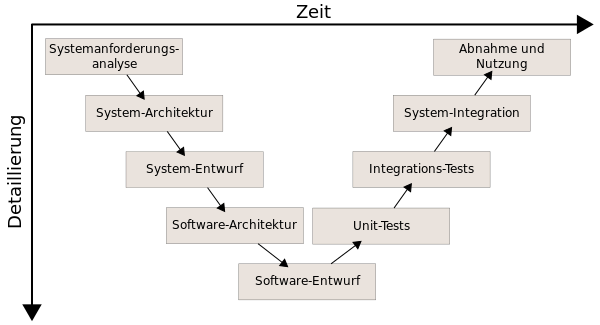
\includegraphics[width=0.8\textwidth]{vmodell}
	\caption{V-Modell, \cite{wiki:vmodellimage}}
\end{figure}

\subsubsection{Komponententest}
Der Komponententest, oder auch Unit-Test genannt, ist ein Test der die kleinste Einheit testen. Dies kann eine Funktion, eine Klasse, ein Unterprogramm oder ein Programm sein. Diese Tests werden typischerweise von den Entwicklern selbst definiert und auch automatisiert. Diese Tests testen dann die fachliche Korrektheit von Teilergebnissen und der technischen Lauffähigkeit der zu testenden Einheit.
\subsubsection{Integrationstest}
Ein Integrationstest testet die Zusammenarbeit voneinander abhängiger Komponenten. Dieser ist jeweils umfangreicher wie ein Unit-Test. Mit diesem werden komplette Abläufe simuliert und die Ergebnisse auf die Richtigkeit überprüft. Je nach Grösse des Projektes werden diese Tests automatisiert.
\subsubsection{Systemtest}
Ein Systemtest testet im Vergleich zum Integrationstest nicht nur die Zusammenarbeit von abhängigen Komponenten sondern gleich das gesamte System. Dabei werden alle funktionalen und nicht-funktionalen Anforderungen getestet. Dieser läuft im Normalfall mit Testdaten auf einem Testsystem ab. Dabei wird die Umgebung des Kunden simuliert.
\subsubsection{Abnahmetest}
Der Abnahmetest ist die letzte Teststufe. Hier wird eine Abnahme der Software simuliert und von Grund auf aufgesetzt, so wie der Kunde es machen wird, wenn er die Software erhält. Ist dieser Test erfolgreich, ist die Software bereit zur Auslieferung.
\cite{wiki:Softwaretest}
\subsection{ISO/IEC 9126}
Um eine Softwarequalität zu testen, gibt es verschiedene Qualitätsmerkmale. Der ISO-Norm 9126 stellt dabei eines von mehreren Modellen dar.
\begin{figure}[H]
	\centering
	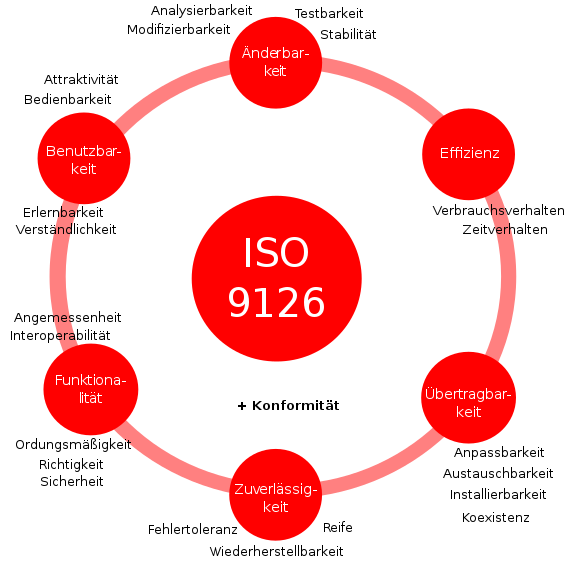
\includegraphics[width=0.6\textwidth]{isonorm}
	\caption{ISO-Norm 9126, \cite{wiki:ISOimage}}
\end{figure}
Dabei gibt es verschiedene Merkmale, welche die Qualität bestimmen.
\subsubsection{Änderbarkeit/Wartbarkeit} 
Dieser Punkt ist vor allem für die Programmierer wichtig. Dabei werden mehrere Punkte bewertet wie der Aufwand, welcher benötigt wird, um Verbesserungen, Änderungen an der Umgebung oder an den Anforderungen der Software zu realisieren. Dabei werden Punkte wie Analysierbarkeit, Modifizierbarkeit, Stabilität oder Testbarkeit berücksichtigt.
\subsubsection{Benutzbarkeit}
Die Benutzbarkeit wird durch den Aufwand, welcher die Software vom Benutzer fordert gemessen. Dieser Aufwand lässt sich in Punkten wie Bedienbarkeit, Erlernbarkeit, Konformität und Verständlichkeit beurteilen.
\subsubsection{Effizienz}
Wie gut kann eine Software mit den verfügbaren Mittel umgehen? Dabei spielen Zeit, aber auch die benötigten Ressourcen wie Festplattenspeicher oder die getane Arbeit eine Rolle.
\subsubsection{Funktionalität} 
Decken die Funktionalitäten die Anforderungen an die Software? Dabei spielen auch Sicherheit und Konformität eine Rolle. Ebenfalls wird das Zusammenspiel mit anderen Systemen und Einhalten von Gesetzten und Normen gewertet.
\subsubsection{Übertragbarkeit} 
Funktioniert die Software auch auf anderen Umgebungen. Dabei wird zwischen Softwareumgebung (z.B. Betriebssystem), Hardwareumgebung (verschieden Computer) und organisatorischer Umgebung unterschieden. So ist es für eine Software von Vorteil, wenn sie nicht auf ein Unternehmen, sondern auf eine Branche massgeschneidert wird. Ebenfalls wird gemessen, ob die Software sich mit anderen Software parallel funktionieren kann oder nicht.
\subsubsection{Zuverlässigkeit} 
Hier sind Punkte wichtig wie die Lauffähigkeit auf Zeit. Oder ob eine gewisse Fehlertoleranz geduldet wird, oder die Software bei einer Nichteinhaltung einer Spezifikation gleich abstürzt. Auch zählen Kriterien wie die Versagenshäufigkeit durch fehlerhafte Zustände.
\cite{wiki:ISO}

\subsection{Good Practice vs. Bad Practice} \label{goodvsbad}
Wie ich bereits erläuterte, sind Tests der Grund, weshalb wir unseren Code überhaupt ändern können. Damit die Tests uns aber dabei unterstützte, gibt es zwei grundlegende Fragen an die Tests.
\begin{itemize}
\item \enquote{Wirst du versagen (oder durchlaufen), wenn ich meinen Code ändere?}
\item \enquote{Ist das ein guter Grund für dich, zu versagen (oder durchzulaufen)?}
\end{itemize}
Ist die Antwort auf die zweite Frage Nein, dann haben wir einen schlechten Test. Er kostet uns Zeit, da wir ihn entweder bei trivialen Änderungen anpassen müssen, oder er lässt uns bei Fehlern im System im Stich.
\subsubsection{Good Practices} \label{Good Practices}
Ein guter Test hat fünf Regeln, welche er einhalten muss. Die Regeln heissen F.I.R.S.T., was für Fast, Isolated, Repeatable, Self-Verifying und Timely steht. Die folgenden Regeln sind primär auf Unittests bezogen, können aber zum Teil auch für Integrationstests angewendet werden.
\paragraph{Fast - Schnell}
Ein Test soll schnell sein. Je schneller der Test, desto mehr wird er ausgeführt. Die Idee dahinter ist, entweder die Tests während der Entwicklung im Hintergrund laufen zu lassen, oder vor dem Check-In eine Testumgebung laufen zu lassen. Hier kann mit schnellen Tests Zeit gewonnen werden. Besonders Zeitintensiv sind Zugriffe ins Internet, auf die Festplatte oder auf grössere APIs. Diese müssen, wenn möglich, umgangen oder gemockt werden.
\paragraph{Isolated - Getrennt}
Ein Test darf nicht von anderen Tests abhängig sein. Müssen die Tests in einer bestimmten Reihenfolge ausgeführt werden, ist das ein Warnhinweis das etwas nicht stimmt. Sind die Tests voneinander abhängig, können Änderungen an einem Test weitere Tests anschlagen lassen. Deshalb sollte Abhängigkeiten dringendst vermieden werden. Auch sollte ein Test nur eine Fehlerquelle haben. Das bedeutet auch, dass ein Test nur etwas testen soll. So kann die Fehlerquelle gleich anhand vom Test erkannt werden und weitere Untersuchungen werden erspart.
\begin{lstlisting}[language=Java, caption={Schlechtes Beispiel}]
@Test
public void testAvailability() {
	source.checkOut(TODAY);
	assertFalse(source.isAvailable());

	source.checkIn(TOMORROW);
	assertTrue(source.isAvailable());
}
\end{lstlisting}
Hier werden gleich zwei Funktionen in einem Test getestet. Dies sollte man in zwei Tests aufteilen.
\begin{lstlisting}[language=Java, caption={Gutes Beispiel}]
@Test
public void isNoLongerAvailableAfterCheckout() {
	source.checkOut(TODAY);

	assertFalse(source.isAvailable());
}

@Test
public void isAvailableAfterCheckin() {
	source.checkOut(TODAY);
	source.checkIn(TOMORROW);
 	
	assertTrue(source.isAvailable());
}
\end{lstlisting}
Wenn hier ein Test fehlschlägt, dann kann man den Fehler klar einer Methode zuordnen.
\paragraph{Repeatable - Wiederholbar}
Ein Test sollte immer das gleiche Resultat erhalten. Egal wie viele Male er ausgeführt wird. Einige Indizien weisen auf potentielle Probleme hin.
\begin{itemize}
\item Statische Daten oder andere nicht bereinigte In-Memory-Konstrukte
\item Volatilität externer Services (z.B. Dateisystem, Datenbank, Webservices, API-Aufrufe)
\item Unkontrolliertes Verhalten durch falsche Verwendung von Threads/Prozessen
\item Abhängigkeit von einer nicht initialisierten (oder langsam initialisierenden) lokalen Klasse
\item Überspezifikation (z.B. Vergleich ganzer Bildschirmbilder oder HTML, wenn nur ein kleiner Teil des Ergebnisses interessant ist)
\end{itemize}
\paragraph{Self-Verifying - Selbstüberprüfend}
Ein guter Test hat ein eindeutiges Testresultat. Entweder ist er erfolgreich oder der Test schlägt an. Deshalb muss ein Test selber eine eindeutige Überprüfung machen. Läuft diese durch, gehen die Programmierer davon aus, dass alles noch funktioniert. 
\begin{lstlisting}[language=Java, caption={Schlechtes Beispiel}]
@Test
public void createReport() {
	Catalog catalog = new Catalog();
	catalog.add(new Holding(BookTestData.AGILE_JAVA));
	catalog.add(new Holding(BookTestData.JAWS));
	catalog.add(new Holding(BookTestData.THE_TRIAL));
 	
	InventoryReport report = new InventoryReport(catalog);
	System.out.println(report.allBooks());
}
\end{lstlisting}
Hier wird davon ausgegangen, dass der Programmierer die Konsolenausgabe liest und selber auf Fehler überprüft. Das dies passiert ist aber eher unwahrscheinlich. Schliesslich gehen die Anzahl automatischer Tests bei grösseren Projekten schnell man in den Tausenderbereich.
\begin{lstlisting}[language=Java, caption={Gutes Beispiel}]
@Test
public void createReport() {
	Catalog catalog = new Catalog();
	// ...
	InventoryReport report = new InventoryReport(catalog);
	assertThat(report.contains(BookTestData.AGILE_JAVA.getClassification());
	// ...
}
\end{lstlisting}
Bei diesem Beispiel sieht man, dass die Richtigkeit vom Test selber überprüft wird.
\paragraph{Timely - Zeitgereicht}
Ein Test sollte immer zusammen mit dem Produktivcode geschrieben werden. Dafür gibt es zwei verschiedene Methoden. Zum einen gibt es die TDD-Methode (Test-Driven Development), bei der man den Test schon vor der eigentlichen Implementierung schriebt. Und dann gibt es die TAD-Methode (Test-After Development), bei der man den Test nach der abgeschlossenen Entwicklung schreibt. Der Vorteil von TDD ist, dass man so gleichzeitig auch die Spezifikationen des Codes festlegt. Natürlich will man das mit TAD auch erzielen, in der Praxis funktioniert das aber eher weniger. Man neigt eher dazu, den Code nur zu verifizieren, statt zu spezifizieren. 
\cite{web:unittestsfirst}
\subsubsection{Bad Practices}
Um schlechte Tests zu vermeiden, gibt es einen guten Merksatz: Binde deine Tests nicht an Implementierungsdetails. Das bedeutet so viel wie, man soll das Resultat überprüfen, nicht den Weg zum Resultat. Der Weg kann und darf bei einem Objekt ändern, ohne dass sich für Benutzer der Klasse was ändert.
\paragraph{Keine privaten Methoden testen}
Sachen, die man nicht machen soll, sind private Methoden testen. Vielmehr sollten die öffentlichen Methoden, welche die privaten Methoden aufrufen getestet werden. Funktionieren diese korrekt, dann funktionieren auch die privaten Methoden korrekt. Schliesslich definieren die öffentlichen Methoden die Funktionen einer Klasse. Was die Klasse Intern macht, geht nur die Klasse etwas an. So kann die Klasse intern geändert werden und man hat immer noch die Kontrolle, ob alles korrekt funktioniert.
\paragraph{Keine privaten Methoden überschreiben}
Private Methoden sollten nicht für Testzwecke überschrieben werden. Öffentliche Methoden haben einen klar definierten Auftrag, welcher man für Testzwecke auch simulieren kann. Private Methoden dagegen haben keinen klaren Auftrag und den Auftrag, den sie haben, kann jederzeit ändern. Auch bringt das die Gefahr, dass der Test trotz Fehler durchläuft. So etwa, wenn eine private Methode umgeschrieben wurde und nun andere Werte zurückgibt. Der Test weiss nichts davon, denn die echte private Methode wurde noch nie aufgerufen, nur jeweils die Simulation. Und der Entwickler, welcher die private Methode anpasste, denkt sich nur, dass er den Test nicht anpassen muss, da er sowieso nur eine private Methode geändert hat. Und die Tests der öffentlichen Methoden laufen ja auch durch.
\paragraph{Keine Konstruktoren testen}
Konstruktoren sollten nicht getestet werden. Den diese können sich ändern. Hier ein kleines Beispiel:
\begin{lstlisting}[language=Java, caption={Klasse Auto}]
public class Car {
	private Engine engine;
	
	public Car() {
		engine = new Engine();
	}
	
	public Engine getEngine() {
		return engine;
	}
}
\end{lstlisting}
\begin{lstlisting}[language=Java, caption={Testklasse}]
@Test
public void testCarConstructor() {
	Car car = new Car();
	Engine engine = ReflectionHelper.getField("engine", car);
	assertNotNull(engine);
}
\end{lstlisting}
Hier bei diesem Beispiel wird getestet, ob der Motor beim Initialisieren vom Auto auch initialisiert wird. Dieser Test funktioniert auch. Wenn man die Klasse Car aber nun folgendermassen anpasst, gibt es Probleme.
\begin{lstlisting}[language=Java, caption={Klasse Auto mit Lazyloading}]
public class Car {
	private Engine engine;
	
	public Car() {
	}
	
	public Engine getEngine() {
		if(engine == null) {
			engine = new Engine();
		}		
		return engine;
	}
}
\end{lstlisting}
Der Motor des Autos wird erst initialisiert, wenn der Motor gebraucht wird. Dies kann aus Performance-technischen Gründen sein. Der Test schlägt nun aber fehl, obwohl das Auto immer noch gleich funktioniert. Deshalb sollte man nicht den Konstruktor testen, sondern nur die öffentlichen Methoden. Hat man nun aber mehrerer Konstruktoren und will wissen ob alle funktionieren, dann kann man das auf folgende Variante tun. Die Tests der öffentlichen Methode werden mit mehreren Instanzen der Klasse ausgeführt. Jede Instanz wird durch einen anderen Konstruktor instanziiert. So sieht man, ob alle Konstruktoren ein korrektes Verhalten hervorrufen.
\cite{web:badpractices}
\paragraph{AssertTrue mit Wertevergleiche}
Leserlicher Code zu produzieren ist eines der wichtigsten Ziele der Programmierer. Dazu gehören intuitive Namensgebungen und einfache Operationen. So kann man auch beim Testen einige Sachen unnötig verkomplizieren, wie zum Beispiel folgendes Beispiel.
\begin{lstlisting}[language=Java, caption={assertTrue falsch eingesetzt \cite{web:abawikijunit5}}]
//Schlechtes Beispiel
Object o = dataProvider.getValue(...);
Assertions.assertTrue(o != null && o instanceof AbaNumber);
Assertions.assertTrue(((AbaNumber)o).equals(AbaNumber.valueOf(4)));

//Gutes Beispiel
Object o = dataProvider.getValue(...);
Assertions.assertNotNull(o);
Assertions.assertEquals(AbaNumber.valueOf(4), o);
\end{lstlisting}
Ein \texttt{assertTrue} sollte nie Vergleiche oder logische Operationen enthalten. Den dafür gibt es extra andere Testmethoden. Für Vergleiche stehen die Methoden \texttt{assertEquals} und \texttt{assertNotEquals} zur Verfügung. Statt logische Operationen zu verwenden, macht man lieber mehrere \texttt{assertTrue}- oder \texttt{assertFalse}-Aufrufe.
\paragraph{AssertTrue(false)}
Eine falsche Verwendung von \texttt{assertTrue} ist, wenn man den Parameter \texttt{false} mitgibt. Dieser Aufruf ist gleichbedeutend wie der Aufruf \texttt{fail}. Diese Methode sagt mehr aus. Sieht man einen Aufruf der fail-Methode, dann weiss man, dass der Test an dieser Stelle fehlschlägt. Sieht man dagegen ein \texttt{assertTrue(false)}, führt dies mehr zur Verwirrung. Man weiss nicht, ob es hier sich um ein Versehen handelt oder der Test anschlagen soll. Dasselbe gilt natürlich auch für \texttt{assertFalse(true)}, welches man auch ab und zu im Code findet.
\begin{lstlisting}[language=Java, caption={assertTrue(false) und fail()}]
//Schlechtes Beispiel
try {
	mHandler.validateAccount(data);
	Assert.assertTrue(false);
} catch (AFWHandlerException e) {
	Assert.assertEquals(e.getMessage(), "Konto ungueltig");
}

//Gutes Beispiel
try {
	mHandler.validateAccount(data);
	Assert.fail();
} catch (AFWHandlerException e) {
	Assert.assertEquals(e.getMessage(), "Konto ungueltig");
}
\end{lstlisting}
\paragraph{DeleteAllRecords}
Dieser Fall ist zwar Abacus-spezifisch, aber dennoch wichtig. Und zwar ist das ein Fehler der sehr viel Zeit kosten kann. Wird in einem Test ein \texttt{deleteAllRecords()} auf einer grossen Tabelle aufgerufen, braucht das enorm viel Zeit. Besser ist es, wenn man die benötigten Datensätze entweder dazu fügt oder einfach bearbeitet. Ein Warnzeichen für ein vergehen ist, wenn ein Test überraschend lange braucht. \cite{web:abawikijunit5}
\begin{lstlisting}[language=Java, caption={}]
//Schlechtes Beispiel
table.deleteAllRecords(null);
table.clear()

table.setfTYP(1);
table.setfCODE("319");
table.setfSATZ(AbaNumber.valueOf(8.0));
table.save(null);

//Gutes Beispiel
table.clear();
table.setIndex_2Fields(1, "319");
table.findEqual(USTConst.IDX_INDEX_2);

table.setfTYP(1);
table.setfCODE("319");
table.setfSATZ(AbaNumber.valueOf(8.0));
table.save(null);
\end{lstlisting}

\section{Testen in der Abacus} \label{Testen in der Abacus}
Hier in der Abacus haben wir verschiedene Arten, wie wir die Software testen.
\subsection{Das Testen aus der Sicht der Supporter}
Die folgende Theorie ist sehr technischlastig und aus der Sicht der Programmierer. Aber was denkt unser Support über das Testen? Schliesslich leisten sie auch einen grossen Teil an der Qualitätssicherung unserer Software. Um dieser Frage nachzugehen, habe ich ein Interview mit Alina Engelmann, Mitarbeiterin im Support der Finanzbuchhaltung, geführt.
\begin{description}
\item[Was kommt dir in den Sinn, wenn du das Wort \enquote{Testen} hörst?] Für mich bedeutet das, dass die Programmierer etwas am Programm geändert oder einen Bug behoben haben und wir dies im Support testen, ob alles korrekt funktioniert. So wird es ja auch ausgeliefert und die Kunden wollen keine fehlerhaften Versionen.
\item[Was für Testarten habt ihr im Support?] Ich persönlich kenne die Jiras und die Checklisten. Bei den Jiras testen wir die Erneuerung, Bug oder was sonst draufsteht und die Checklisten müssen wir abarbeiten. Zum Beispiel ob das Drucken funktioniert. Die Checklisten decken vor allem zentrale Komponenten ab.
\item[Wie unterscheiden sich Checklisten und Jiras?] Checklisten sind von Jahr zu Jahr dieselben. Die Jiras dagegen sind ganz unterschiedlich. Dort kann alles kommen. Zum Beispiel werden die Kundenwünsche als Jiras erfasst und von Zeit zu Zeit auch mal gelöst. Dann müssen diese auch getestet werden.
\end{description}
Das ganze Interview ist in der Abgabedatei enthalten.
\subsection{Möglichkeiten und Hilfsmittel}
Damit wir effizient Testen können, gibt es verschiedene Hilfsmittel in der Firma. Einige sind spezifisch für die Programmierer, andere für alle.
\subsubsection{Hilfsmittel für Programmierer}
\paragraph{JUnit}
JUnit ist ein Framework für Java, welches hilft, Tests zu automatisieren. Mithilfe dieses Frameworks können wir Methoden, welche eine Funktion des zu testenden Objekts testet, als eine Testmethode definieren. Läuft der Test durch war er entweder erfolgreich oder er hat Fehler. Es gibt nur diese zwei Ergebnisse.
\paragraph{Bamboo}
Der Bamboo ist eine Software, welche für uns die Tests managt und laufen lässt. Diese werden jeweils auf Servern laufen gelassen und uns anschliessend eine Zusammenfassung der Ergebnisse erstellt. Der Bamboo lässt die Tests auch jede Nacht einmal durchlaufen, so dass wir allfällige Fehler spätestens einen Tag später bemerken.
\paragraph{Mockito}
Mockito ist eine Bibliothek für Java, welches uns das Testen vereinfacht. Mithilfe dieser Bibliothek lassen sich Klassen mocken, was so viel wie simulieren heisst. So müssen wir eine Klasse nicht Instanziieren, sondern können sie nach unseren Vorgaben simulieren lassen. Dies kann Tests zum einen vereinfachen und auch Performance-technische Optimierung bringen. Auch hat man die Möglichkeit die Objekte zu überwachen. So kann man überprüfen, ob gewisse Methoden mit den korrekten Parametern aufgerufen wurden oder die Methoden überhaupt aufgerufen wurde.
\paragraph{ReflectionHelper}
Der ReflectionHelper ist eine Klasse, welche ebenfalls für das Erstellen von Testklassen benötigt wird. Er bietet verschiedene Methoden an, um Felder von Objekten mit eigenen Instanzen auszutauschen oder gewisse Methoden aufzurufen. In Kombination mit Mockito lassen sich die Objekte stark überwachen und die verrichtete Arbeit leichter überprüfen.
\subsubsection{Hilfsmittel für alle}
\paragraph{AbaMovie}
AbaMovie ist eine Funktion, mit welcher Aktionen, welche auf dem UI gemacht werden, gespeichert werden können. Diese kann man dann Wiedergeben. So können ganze Abläufe aufgenommen und regelmässig abgespielt werden, um zu überprüfen, dass noch alles funktioniert. So werden ganze Systemtests automatisiert.
\paragraph{AbaTest}
AbaTest ist ein internes Programm, über welches virtuelle Maschinen bestellt werden können. Dies wird vor allem zum Testen von Änderungen benötigt. Der VM kann man einige Parameter mitgeben, wie etwa das Betriebssystem, die Datenbank, die Arbeitsspeichergrösse oder die Abacusinstallation.

\subsection{Teststufen}
Die Gliederung des V-Modells kann gleich auf die einzelnen Tests angewendet werden.
\subsubsection{Komponententest}
Die Komponententests werden von uns Entwickler beim Lösen des Fehlers gleich dazugeschrieben. So wird versucht, den Fehler in Zukunft zu vermeiden. Bei Neuentwicklungen werden jeweils neue Tests geschrieben, die das Ziel haben so viel der Software abzudecken wie möglich. Dabei gilt die Faustregel, dass für jede Serverklasse ein Test erstellt werden muss, für Clientklassen aber nicht. Tests, wie ob ein Knopf auf dem UI ist oder nicht wären zu umständlich. Und zudem testen wir das UI anders, mehr dazu später. Wenn man aber komplizierte Logik in einer Clientklasse hat, dann muss auch diese getestet werden. Diese Unittests werden mit dem Framework JUnit geschrieben. Diese werden, wie der Sourcecode auch, ins Subversion-System geladen und von dort aus auf den Bamboo-Agenten. Dieser führt alle Tests durch und tragt uns alle Fehler zusammen. Diese laufen jeden Tag mindestens einmal durch. Zusätzlich helfen uns dabei Tools wie Sonarqube, welche die Codeabdeckung der Tests überprüft und potentielle Fehlerquellen im Code sucht.
\begin{figure}[H]
	\centering
	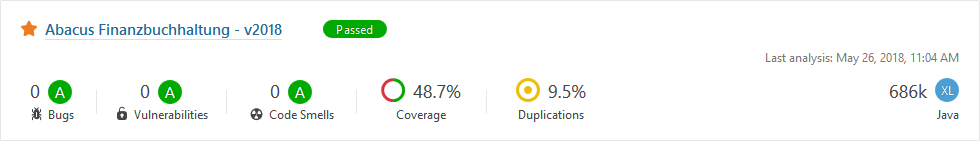
\includegraphics[width=\textwidth]{sonarqube}
	\caption{Eine Auswertung von Sonarqube vom Projekt Abacus Finanzbuchhaltung - v2018}
\end{figure}
\subsubsection{Integrationstest}
Die Integrationstests werden wie die Unittests von uns Entwicklern geschrieben. Wird ein grösseres neues Feature geschrieben oder es gibt Änderungen an einer grösseren Funktion dann werden Integrationstests geschrieben, welche das Zusammenspiel mehrerer Klassen oder Komponenten testet. Auch diese Laufen auf dem Framework JUnit und sind automatisiert. Wird eine Entwicklung abgeschlossen, wird die Umsetzung zuerst vom Entwickler gründlich getestet. Anschliessend wird die Aufgabe einem anderen Entwickler gegeben, damit dieser die Entwicklung noch von einer anderen Sicht aus testen kann. So wird die Entwicklung jeweils von zwei Personen gleich im System getestet. Bestätigt der zweite Entwickler, dass die Änderungen korrekt sind, wird die Aufgabe am Support übergeben, welcher ebenfalls die Änderung nochmals überprüft. So soll verhindert werden, dass neue Änderungen das System kaputt machen. 
\begin{figure}[H]
	\centering
	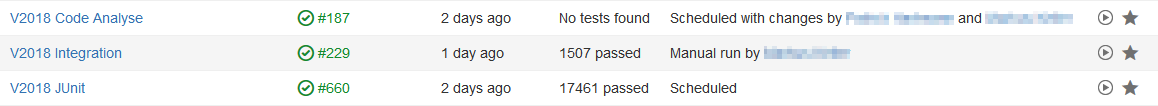
\includegraphics[width=\textwidth]{bamboo}
	\caption{Eine Auswertung von Bamboo vom Projekt v2018 Finanzbuchhaltung}
\end{figure}
\subsubsection{Systemtest}
Um das ganze System zu Testen haben wir die sogenannten AbaMovies. Das Prinzip ist ganz einfach. Man klickt im Programm umher und verändert zum Beispiel Daten. Dies wird aufgenommen und kann jederzeit wieder wiedergeben werden. Nun werden so ganze Abläufe aufgenommen. Diese werden, wenn möglich jeden Tag laufen gelassen. Wenn nun etwas nicht mehr so funktionierte, wie es mal hat, laufen diese Tests nicht mehr durch. Dasselbe passiert, wenn auf einmal andere Daten daherkommen wie früher. So wird die ganze Software täglich auch noch aus einer anderen Sichtweise getestet. Zusätzlich dazu haben wir auch Tests welche manuell ausgeführt werden müssen. Das sind Checklisten, welche einen Ablauf genau beschreiben. Bevor eine Auslieferung aussteht, müssen diese Checklisten einmal durchgespielt werden.
\subsubsection{Abnahmetest}
Für die Abnahmetests haben wir extra eigene Kunden. Diese Testen die Beta-Version unserer Software, erhalten diese als Gegenleistung dafür zu einem günstigeren Preis. Diese Kunden testen die Software im Produktiveinsatz. Gibt es bei den Systemen dieser Kunden Probleme, wird der Entwicklung das gemeldet und korrigiert, bevor die Software an alle Kunden gelangt.

\subsection{Testen verschiedener Qualitätsmerkmale}
\subsubsection{Änderbarkeit/Wartbarkeit} 
Dieser Punkt lässt sich nicht so einfach testen, da er mit der Softwarearchitektur zusammenhängt. Das heisst aber nicht das dieser Punkt vernachlässigt wird. Es werden stetig neue Frameworks eingeführt und alte abgelöst, um die Einfachheit, Testbarkeit und Stabilität des Codes zu gewähren.
\subsubsection{Benutzbarkeit} 
Auch für die Benutzbarkeit haben wir keine Tests. Jedoch haben wir einen Experten im Haus. Er ist die Ansprechperson, wenn es um den Bau von effizientem UI, welches ansprechend und einfach erlernbar sein soll, geht. Er hat das Ziel, das UI für die Kunden so zu verbessern, dass die Benutzbarkeit steigt.
\subsubsection{Effizienz}
Die Effizienz liegt in den Händen der Programmierer. Natürlich wird die Software, wenn möglich so programmiert, dass wir ein möglichst sparsamen Umgang mit den Ressourcen haben. So werden offene Tabellenverbindungen zentral gespeichert, damit nicht jedes Programm selber eine Tabelle öffnet. Auch haben wir schon Rückmeldungen von Kunden bekommen, welche zeitliche Probleme mit der Installation haben, da sie viele Daten zu verarbeiten hatten. Diese Probleme werden dann individuell angeschaut. Ein aktives Testen der Effizienz gibt es so aber bei uns nicht.
\subsubsection{Funktionalität} 
Die Funktionalität ist das Hauptmerkmal unseres Testens in der Firma. So sind die Unittests, Integrationstests und Systemtests primär da, dies zu gewährleisten. Ändert eine Funktionalität unabsichtlich durch eine andere Änderung, wird dies in den meisten Fällen durch diese Tests aufgedeckt.
\subsubsection{Übertragbarkeit} 
Damit wir die Gewährleistung unserer Software auch auf anderen Systeme gewährleisten können, haben wir die Möglichkeit die gelösten Aufgaben auf fremden Systemen zu testen. So können einfach VMs mit verschiedenen Betriebssystemen automatisch generiert werden. Ebenso bieten wir unsere Software zurzeit mit zwei verschiedenen Datenbanken an. Damit dies sicher funktioniert, laufen alle Unittests auf zwei Installationen mit jeweils unterschiedlicher Datenbank. Auch wird in der Abacus auf Windows, OSX und vereinzelt auf Linux entwickelt. So werden täglich die verschiedenen Systeme passiv getestet.
\subsubsection{Zuverlässigkeit} 
Die Zuverlässigkeit testen wir vor allem mit unseren Beta-Kunden. Diese Testen die Installation produktiv über längere Zeit. Damit wir keine Fehler in die Daten bekommen, werden die Daten jeweils UI-seitig sowie Serverseitig validiert und bei falschen Eingaben dem Kunden eine sprechende Fehlermeldung ausgegeben.


\subsection{Testdaten in der Abacus} \label{Datenspeicherung}
Daten spielen in den Tests eine zentrale Rolle. Dank ihnen lassen sich die Resultate der Tests überprüfen. Wie wir die Daten den zu testenden Klassen übergeben unterscheidet sich hier in der Firma. Deshalb gibt es hier eine Auflistung der fünf Methoden, welche genutzt werden. 
\subsubsection{Manuelles Aufsetzen von Objekten}
Nicht selten findet man in Tests, dass die Datenobjekte manuell aufgesetzt werden. So etwa in der folgenden Testmethode. Dabei wird das Data-Objekt leer instanziiert und anschliessend, über die vorhandenen Set-Methoden abgefüllt.
\begin{lstlisting}[language=Java, caption=Testmethode mit manuell aufgesetztem Datenobjekt]
@Test
public void testSaveNewAccount() {
	KONErfassenData data = new KONErfassenData();
	data.setEnterprise(0);
	data.setNr(1234567L);
	data.setName("Mein Konto");
	data.setIso("CHE");
	data.setClassrefid(AbaNumber.valueOf(2));
	// ...
	ObjectContainer container = new ObjectContainer(ElementType.NEW, data, null, null);
	KONSaveletData saveletData = new KONSaveletData(container);
	invokeAllTransactionReal(saveletData);
	// ...
}
\end{lstlisting}
\paragraph{Vorteile}
\begin{itemize}
\item Praktisch bei Klassen, welche genauso ein Datenmodell brauchen.
\item Vorhandene Daten sind auf einen Blick ersichtlich
\item Es müssen nur Daten eingetragen werden, welche für den Test auch benötigt werden.
\end{itemize}
\paragraph{Nachteile}
\begin{itemize}
\item Müssen viele Felder abgefüllt werden, hat man viel Schreibarbeit.
\item Nicht geeignet für Klassen, welche die Daten von der Datenbank holen.
\end{itemize}
\subsubsection{Daten von Mandanten}
Eine weitere Variante, welche man häufig sieht, ist das Laden der Daten direkt auf Mandanten. Hier wird z.B. ein Datensatz auf der HJO angelegt. Im späteren Verlauf wird der Test die HJO wieder öffnen und nach dem Datensatz suchen. Dabei wird hier gleich der Vorteil ausgenutzt, dass die abhängigen Daten, wie das Konto 1010100 bereits existiert und dies nicht auch noch erfasst werden muss.
\begin{lstlisting}[language=Java, caption=Testmethode mit Daten vom Mandant]
@Mandant(300)
@Test
public void testGetAllEnterprises() {
	HJO hjo = new HJO(mFGI);
	hjo.open(OpenMode.READWRITE);
	hjo.clear();
	hjo.setIndex_1Fields(1010100L, AbaDate.EMPTY, 2011, HJOConst.SOLLIST_0, 0, 1);
	hjo.save(TransactionUtil.NO_TRANSACTION);
	// ...
}
\end{lstlisting}
\paragraph{Vorteile}
\begin{itemize}
\item Daten bereits vorhanden
\item Praktisch bei Klassen, welche auf die Datenbank zugreifen
\item Kleiner Aufwand zum Erstellen der Daten
\end{itemize}
\paragraph{Nachteile}
\begin{itemize}
\item Neue Thematiken haben keine Testdaten
\item Abhängigkeit an Mandant
\item Testdaten nicht anpassbar
\end{itemize}

\subsubsection{Datenklassen} \label{Datenklasse}
Bei dieser Variante ruft man eine statische Methode einer solchen Klasse auf, welche anschliessend Daten in die Datenbank lädt. Alternativ kann die Klasse vor dem Test mit der Annotation @LoadDataClass vor dem Test geladen werden.
\begin{lstlisting}[language=Java, caption=Beispiel einer Datenklasse]
private static void fillTableKON(GlobalInterface gl) throws Exception {
	KONBase table = new KONBase(gl);
	table.open(OpenMode.READWRITE);
	table.deleteAllRecordsSafe(TransactionUtil.NO_TRANSACTION);

	//record 1
	table.clear();
	table.setfNAME("Kasse");
	table.setfNR(1000L);
	table.setfWAEHR("SFr");
	table.setfKLASSE_BI("A");
	table.setfKART("0");
	table.setfISO("CHF");
	table.setfKST("0");
	// ...
	
	table.save(null);
	
	//record 2
	table.clear();
	table.setfNAME("Vorsteuer auf Materialaufw. und Dienstl.");
	table.setfNR(1170L);
	table.setfWAEHR("SFr");
	table.setfKLASSE_BI("A");
	table.setfKART("0");
	table.setfISO("CHF");
	table.setfKST("0");
	// ...

	table.save(null);
	
	// ...
\end{lstlisting}
\paragraph{Vorteile}
\begin{itemize}
\item Für mehrere Tests verwendbar
\item Kleiner Aufwand zum Laden von Daten
\item Praktisch für Klassen, welche auf die Datenbank zugreifen
\item Geringer Aufwand um Testdaten anzupassen
\item Lässt sich aus Mandantdaten generieren
\end{itemize}
\paragraph{Nachteile}
\begin{itemize}
\item Abhängigkeit von der Testklasse
\end{itemize}

\subsubsection{Datenpaket} \label{Datenpaket}
Bei einem Datenpaket ist ein ZIP-File mit der Endung bin im selben Ordner. Das Paket kann nun vor einem Test mit der Annotation @LoadData angegeben werden. Diese enthalten Daten, welche nun ins System zurückgeladen werden.
\begin{lstlisting}[language=Java, caption=Beispiel eines Datenpaketes]
@Test
@LoadData({"TestGb0Betraege.bin"})
public void testKursausgleichGb0Betraege() {
	// ...
	AbaNumber betrGB0 = mockFVDE.getGB0KursausgleichBetr(0, kon, data, 1.25, false);
	Assertions.assertTrue(betrGB0.equals(-15500));
}
\end{lstlisting}
\begin{lstlisting}[language=XML, caption=Inhalt einer Datei des Datenpaketes]
<?xml version='1.0' encoding='UTF-8'?>
<table name='45646.fibu.e13'>
  <insert recnum='1'>
    <field id='DATE' type='Date'>2013-03-01</field>
    <field id='KTO' type='Number'>1021</field>
    <field id='GKTO' type='Number'>1020</field>
    <field id='TEXT' type='String'>usd buchung</field>
    <field id='BETRAG' type='Number'>9000</field>
    <field id='SH' type='String'>S</field>
    <!-- ... -->
  </insert>
  <insert recnum='2'>
    <field id='DATE' type='Date'>2013-12-31</field>
    <field id='BELNR' type='String'>        10</field>
    <field id='KTO' type='Number'>1021</field>
    <field id='GKTO' type='Number'>6891</field>
    <field id='SAM' type='String'>#</field>
    <field id='TEXT' type='String'>Verbuchung Kursausgleich</field>
    <field id='BETRAG' type='Number'>800</field>
    <field id='SH' type='String'>S</field>
    <!-- ... -->
  </insert>
  <!-- ... -->
\end{lstlisting}
\paragraph{Vorteile}
\begin{itemize}
\item Für mehrere Tests verwendbar
\item Kleiner Aufwand zum Laden von Daten
\item Praktisch für Klassen, welche auf die Datenbank zugreifen
\item Lässt sich aus Mandantdaten generieren
\end{itemize}
\paragraph{Nachteile}
\begin{itemize}
\item Grosser Aufwand um Testdaten anzupassen
\item Abhängigkeit vom Datenpaket
\end{itemize}

\subsubsection{Daten mocken}
Eine weitere Variante, welche man aber eher selten antrifft, ist das Mocken der Daten. Dabei wird dem Objekt nur gesagt, welcher Wert für eine gewisse Funktion zurückgegeben werden soll. Daten werden so aber keine gespeichert oder zurückgeladen.
\begin{lstlisting}[language=Java, caption=Beispiel einer gemockten Tabelle]
@Test
public void test_getCallbackValue() {
	// prepare data
	// ...
	SYS sys = Mockito.mock(SYS.class);

	Mockito.when(mDataMap.getGlobalInterface()).thenReturn(getGlobalInterface());
	Mockito.when(mDataMap.getDataSet()).thenReturn(sys);

	// ...

	for (int identifier = 0; identifier < 20000; identifier++) {
		switch (identifier) {
			case MandantenStammDataMap.DRUCKSPRACHE:
			Mockito.doReturn(Language.DE).when(sys).getFibuDruckSprache();
			assertEquals(Language.DE, mDataMap.getCallbackValue(identifier, property));
			Mockito.doReturn(Language.EN).when(sys).getFibuDruckSprache();
			assertEquals(Language.EN, mDataMap.getCallbackValue(identifier, property));
		break;
		case MandantenStammDataMap.MFR_VON_MANDAND:
			Mockito.doReturn(false).when(sys).getMittelflussRechnungGlobal();
			assertEquals(true mDataMap.getCallbackValue(identifier, property));
			Mockito.doReturn(true).when(sys).getMittelflussRechnungGlobal();
			assertEquals(false, mDataMap.getCallbackValue(identifier, property));
		break;
\end{lstlisting}
\paragraph{Vorteile}
\begin{itemize}
\item Man kann gezielt Get-Methoden übersteuern
\end{itemize}
\paragraph{Nachteile}
\begin{itemize}
\item Grosser Schreibaufwand
\item Verhaltensänderungen der Tabelle werden ignoriert, da Methoden übersteuert werden
\item Tabelle muss bei der zu testenden Klasse durch Mock ersetzt werden.
\end{itemize}

\section{Planung} \label{Testmöglichkeiten}
Damit wir die verschiedenen \nameref{Testmethoden} auswerten können, erstelle ich ein Testkonzept, wie ich die verschiedenen Testmethoden am besten miteinander vergleichen kann, sodass am Ende bessere und schlechtere Methoden unterschieden werden können.
\subsection{Testmethoden} 
In den Vorgaben der IPA habe ich verschiedene Testmethoden, welche ich auswerten muss. 
\subsubsection{Grosser änderbarer Mandant}
Es gibt heute schon  grosse Mandanten, mit welchen Tests geschrieben werden können. Diese sind aber nicht modifizierbar. Dies hat primär den Grund, dass Auswertungen getestet werden können. Wenn sich Daten ändern, ändern sich auch das Resultat von Auswertungen, was wiederum die Tests anschlagen lässt. Neu soll ein Mandant erstellt werden, der von allen geändert werden darf um neue Testdaten einzutragen.
\subsubsection{Eingefrorene Mandanten nach Thematik}
Ähnlich wie die heutigen Mandanten, sollen neue Mandanten, auf verschiedene Thematiken zugeschnitten, erstellt und eingefroren werden. Diese könnten dann nicht nur zum Testen verwendet werden, sondern auch beim Bearbeiten von Jiras aus dieser Thematik.
\subsubsection{Mandanten ohne Daten}
Statt das Mandanten die Daten haben, sollen die Testklassen der Tabellen Methoden haben, um Daten aufzusetzen. So können Daten mit einem Methodenaufruf einfach geladen werden. Dabei werden nur Daten für eine Tabelle erstellt. Hier kann zur Vereinfachung das Tool, welches in den Methoden \nameref{Datenklasse} und \nameref{Datenpaket} verwendet werden, eingesetzt werden. 
\subsubsection{Klassen zur Aufsetzung ganzer Thematiken}
Anstatt eines Mandanten, welcher eine ganze Testthematik enthält, sollen Klassen erstellt werden, welche selber eine ganze Testthematik mit zusammenhängenden Daten erstellt. Dabei sind keine Vorgaben, ob ich die Klasse wie in der Methode \Nameref{Datenklasse} generieren lassen will, oder ob ich einen anderen Weg dafür nehme.
\subsection{Bewertung der Methoden}
Um verschiedene Methoden miteinander vergleichen zu können, braucht es einige \nameref{Evaluationskriterien}. Einige sind dabei schon vorgegeben.
\subsubsection{Evaluationskriterien}
\paragraph{Wartung der Tests}
Hier geht es vor allem um den Aufwand bei Änderungen am Code oder der Datenstruktur. Je weniger Aufwand desto besser. 
\paragraph{Wartung des Bamboos}
Damit die Tests durchlaufen, muss der Bamboo gewartet und aktuell gehalten werden. Hier wird der zusätzliche Aufwand gemessen, der bei Verwendung einer anderen Methode entsteht.
\paragraph{Erweiterung der Tests}
Wird eine neue Thematik erstellt oder eine bereits vorhandene Thematik erweitert, muss der neue Code getestet werden. Dieses Kriterium setzt den Aufwand fest, der eine Erweiterung verschiedener Tests bringt.
\paragraph{Unabhängigkeit der Tests}
Beziehen mehrere Tests von der gleichen Quelle ihre Daten, so besteht eine gewisse Abhängigkeit. Hier wird gemessen, wie abhängig die Tests von zentralen Quellen, wie zum Beispiel einem Mandanten sind. Je grösser die Abhängigkeit, desto grösser die Wahrscheinlichkeit, dass Tests durch zentrale Änderungen kaputt gehen können.
\paragraph{Andere Vorteile}
In der Kategorie andere Vorteile gehen verschiedene Punkte ein, welche damit kommen. Beispielsweise könnte ein themenbezogener Mandant die Arbeit an diesem Thema für erleichtern, da schon Daten im System vorhanden sind. 
\paragraph{Performance}
Bei der Performance geht es um die reine Geschwindigkeit des Tests. Wie im Abschnitt \Nameref{Good Practices} schon erwähnt sollte ein Test so schnell wie möglich sein.
\paragraph{Initialaufwand}
Wird ein Test von Grund auf neu erstellt, benötigt das Erstellen von Daten Zeit. Hier wird gemessen, wie viel mehr Zeit dies benötigt.
\subsubsection{Messen der Kriterien}
Damit wir diese Kriterien gleichmässig Messen können, wird für jeden Punkt ein Bewertungsraster definiert. So können am Schluss alle Punkte miteinander verglichen werden. Dabei hat jeder Punkt auch eine Gewichtung. Die letztendliche Punktzahl des Codes wird durch die Formel \(Gewichtung * Punktzahl\) berechnet. Dabei ist das Gesamtresultat die Summe aller Gesamtpunkte der Kriterien.
\begin{equation}
\begin{split}
K = Liste\ aller\ Kriterien\\
n = Anzahl\ Kriterien\\
gew(k) = Gewichtung\ des\ Kriteriums\\
pnkt(k) = Punktzahl\ des\ Kriteriums\\
\displaystyle\sum_{i=0}^{n} gew(K_{i}) * pnkt(K_{i})
\end{split}
\end{equation}
Die Punkteverteilung erfolgt nach dem schweizerischen Notensystem, wobei 1 sehr schlecht und 6 sehr gut ist.

\paragraph{Wartung der Tests}
Die Wartung der Tests messe ich in Zeit. Dabei werde ich bei jeder Testmethode dieselben Tests anpassen und die Zeit dafür stoppen. So habe ich klare Werte, welche ich vergleichen kann. Mit folgender Tabelle werde ich die Ergebnisse benoten. Die Gewichtung setzte ich auf eine drei an, da man nicht allzu oft die Tests warten muss. Wenn man dennoch mal die Tests anpassen sollte, will man natürlich trotzdem nicht, dass es zu lang geht.\\
Damit ich die Wartung der Tests sinnvoll planen kann, erstelle ich hier ein Konzept, was alles geändert werden muss, um die Wartbarkeit zu überprüfen. 
\begin{itemize}
\item Auf den Datensätze der Tabelle \texttt{HJO}, auf welche der Test zugreift, sollen die Felder KST verändert werden.
\end{itemize}
\begin{table}[H]
\begin{tabularx}{\textwidth}{|l|X|X|X|X|X|X|}
\hline
\thead{Punktzahl} & \thead{1} & \thead{2} & \thead{3} & \thead{4} & \thead{5} & \thead{6} \\	\hline
Bedingung & >20 Minuten & <20 Minuten & <15 Minuten & <10 Minuten & <5 Minuten & <3 Minuten \\ \hline
Gewichtung & \multicolumn{6}{c|}{3} \\ \hline
\end{tabularx}
\caption{Bewertungsraster für die Wartung der Tests}
\end{table}

\paragraph{Wartung des Bamboos}
Die Arbeit, welche bei der Wartung des Bamboos vor allem gemacht wird, ist Tabellen der Mandanten updaten oder Windowsinstallationen installieren, wobei Zweiteres uns weniger interessiert. Die Tabellen der verschiedenen Mandanten können alle miteinander aktualisiert werden, sodass ein einzelner Mandant nicht ins Gewicht fällt. Ins Gewicht fällt dafür, dass diese Arbeiten im Durchschnitt einmal wöchentlich und pro Installation separat gemacht werden müssen. So multipliziert sich zusätzliche Wartezeit. Jedoch falle diese ein paar Sekunden pro Mandant relativ klein aus. Deshalb setzte ich die Gewichtung als eine zwei fest.
\begin{table}[H]
\begin{tabularx}{\textwidth}{|l|l|l|l|l|l|X|}
\hline
\thead{Punktzahl} & \thead{1} & \thead{2} & \thead{3} & \thead{4} & \thead{5} & \thead{6} \\	\hline
Bedingung &  &  & 1 Mandant pro Test & 1 Mand. pro Thema & 1 Mandant & Keine Mandanten \\ \hline
Gewichtung & \multicolumn{6}{c|}{2} \\ \hline
\end{tabularx}
\caption{Bewertungsraster für die Wartung des Bamboos}
\end{table}

\paragraph{Erweiterung der Tests}
Werden Themen erweitert oder Fehler geflickt, so werden die vorhandenen Tests meist erweitert. Dabei spielt die Zeit eine wesentliche Rolle. Deshalb wird die Bewertung anhand der Zeit erfolgen, welche ich benötige um eine Anzahl vorgegebener Tests anzupassen. Die Gewichtung wird, da der Fall, dass man Tests erweitern muss häufig vorkommt, auf eine 4 gesetzt. Folgende Tabelle wird mir bei der Auswertung helfen.\\
Hier messe ich die Zeit, welche ich benötige, um die Methoden \texttt{saveAdrLink1}, \texttt{saveAdrLink2} und \texttt{saveAdrLink3} zu testen.
\begin{table}[H]
\begin{tabularx}{\textwidth}{|l|X|X|X|X|X|X|}
\hline
\thead{Punktzahl} & \thead{1} & \thead{2} & \thead{3} & \thead{4} & \thead{5} & \thead{6} \\	\hline
Bedingung & >40 Minuten & <40 Minuten & <20 Minuten & <12 Minuten & <8 Minuten & <5 Minuten \\ \hline
Gewichtung & \multicolumn{6}{c|}{4} \\ \hline
\end{tabularx}
\caption{Bewertungsraster für die Erweiterung der Tests}
\end{table}

\paragraph{Unabhängigkeit der Tests}
Die Unabhängigkeit der Tests ist insofern wichtig, da man andere Tests so ungewollt kaputt machen kann. Die Auswirkungen davon sind meist erst auf dem Bamboo ersichtlich und die Korrektur meist zeitintensiv. Deshalb ist dieser Punkt nicht zu unterschätzen. Die Messung dieses Punktes ist schwer zu realisieren. Deshalb zähle ich die Anzahl Abhängigkeiten von einer Datenquelle. Je weniger Verbindungen zu einer Datenquelle existieren, desto weniger ist der Tests abhängig.
\begin{table}[H]
\begin{tabularx}{\textwidth}{|l|l|l|X|X|X|X|}
\hline
\thead{Punktzahl} & \thead{1} & \thead{2} & \thead{3} & \thead{4} & \thead{5} & \thead{6} \\	\hline
Bedingung & & Tests von überall & eine Testthematik & Tests von einem Programm & eine Testklasse & eine Testmethode \\ \hline
Gewichtung & \multicolumn{6}{c|}{4} \\ \hline
\end{tabularx}
\caption{Bewertungsraster für die Unabhängigkeit der Tests}
\end{table}

\paragraph{Andere Vorteile}
Da andere Vorteile nicht einfach messbar sind, wird dieser Punkt bei jedem Test manuell ausgefüllt und bewertet. Standardmässig gibt es eine eins wobei die Gewichtung auch nur eins ist. Die Gewichtung ist deshalb so gering, weil die wichtigen Punkte schon gemessen werden. Dieser Punkt spielt so nur das Zünglein an der Waage, wenn sich zwei Methoden als ähnlich gut herausstellen.
\begin{table}[H]
\begin{tabularx}{\textwidth}{|l|X|X|X|X|X|X|}
\hline
\thead{Punktzahl} & \thead{1} & \thead{2} & \thead{3} & \thead{4} & \thead{5} & \thead{6} \\	\hline
Bedingung & Standartwert & & & & &  \\ \hline
Gewichtung & \multicolumn{6}{c|}{1} \\ \hline
\end{tabularx}
\caption{Bewertungsraster für andere Vorteile einer Methode}
\end{table}

\paragraph{Performance}
Den Punkt Performance ist dafür wieder einfach messbar. Da ich neue Tests schreibe und nicht bereits ein Referenzwert habe, werde ich die Methoden mit der schnellsten Methode vergleichen. Der prozentuale Unterschied ergibt dann die Punktzahl.
\begin{equation}
\begin{split}
t_{a} = Laufzeit\ mit\ neuer\ Methode\\
t_{b} = Laufzeit\ der\ schnellsten\ Methode\\
dif = \frac{t_{a}}{t_{b}} - 100\% \\
\end{split}
\end{equation}
Dabei hat die Performance eine Gewichtung 4. Zum eine sollte der Test schon schnell sein, dennoch ist es nicht das wichtigste Kriterium.\\
Da die Tests nicht jedes Mal eine identische Zeit haben, werde ich die Tests 5 Mal laufen lassen und dann den Durchschnittswert nehmen.
\begin{table}[H]
\begin{tabularx}{\textwidth}{|l|X|X|X|X|X|X|}
\hline
\thead{Punktzahl} & \thead{1} & \thead{2} & \thead{3} & \thead{4} & \thead{5} & \thead{6} \\	\hline
Bedingung & >100\% & <100\% & <60\% & <20\% & <10\% & 0\%  \\ \hline
Gewichtung & \multicolumn{6}{c|}{4} \\ \hline
\end{tabularx}
\caption{Bewertungsraster für Performance eines Tests}
\end{table}

\paragraph{Initialaufwand}
Der Initialaufwand ist der wahrscheinlich wichtigste Punkt. Den er bestimmt die Zeit, welche wir für neue Tests benötigen. Und dies kommt regelmässig vor. Deshalb erhält dieses Kriterium die Gewichtung sechs. Um die Initialzeit zu messen, werde ich verschiedene Tests erstellen mit den zugehörigen Daten. Die Zeit wird vom Beginn bis zum ersten erfolgreichen Durchlauf gemessen.
\begin{table}[H]
\begin{tabularx}{\textwidth}{|l|X|X|X|X|X|X|}
\hline
\thead{Punktzahl} & \thead{1} & \thead{2} & \thead{3} & \thead{4} & \thead{5} & \thead{6} \\	\hline
Bedingung & >60 Minuten & <60 Minuten & <50 Minuten & <40 Minuten & <30 Minuten & <20 Minuten \\ \hline
Gewichtung & \multicolumn{6}{c|}{6} \\ \hline
\end{tabularx}
\caption{Bewertungsraster für den Initialaufwand}
\end{table}

\subsubsection{Bewertungsmatrix}
\begin{table}[H]
\begin{tabularx}{\textwidth}{|X|c|c|c|}
\hline
\thead{Kategorie} & \thead{Gewichtung} & \thead{Bewertung} & \thead{Gesamtpunktzahl} \\	\hline
Wartung der Tests & 3 & & \\	\hline
Wartung des Bamboos & 2 & & \\	\hline
Erweiterung der Tests & 4 & & \\	\hline
Unabhängigkeit der Tests & 4 & & \\	\hline
Andere Vorteile & 1 & & \\	\hline
Performance & 4 & & \\	\hline
Initialaufwand & 6 & & \\	\hline
\multicolumn{3}{|l|}{Gesamtpunktzahl} & \\ \hline
\end{tabularx}
\caption{Bewertungsraster um die Testmöglichkeiten zu bewerten}
\end{table}

\subsection{Tests} \label{Testmethoden2}
Die Methoden, welche ich für das Testen nehme, werde ich neu schreiben. Als ich den \texttt{KSTErfassenHandler} und den dazugehörigen Test analysierte, fiel mir auf, dass die Methode \texttt{beforeTransaction} wenig Testfälle hat. Deshalb werde ich für die verschiedenen Validierungen Testfälle schrieben. Der Vorteil dazu ist, zum einen kann ich den Punkt Initialaufwand messen, zum anderen bringen die Auswertungen so gleich noch zusätzliche Codeabdeckung. Dabei hat die Methode 16 Fälle, bei welchen die Validierung anschlägt. So ergibt das 16 neue Testmethoden.

\section{Auswertung} \label{Auswertung}
\subsection{Auswertung einzelner Testmethoden}
Um die Gesamtpunktzahl der Methoden zu ermitteln, werden die einzelnen Kriterien nun ausgewertet und anhand der Tabellen die Punkte verteilt. Diese werden in die Bewertungsmatrix eingegeben und die Resultate ausrechnen.
\subsubsection{Grosser änderbarer Mandant}
\begin{description}
\item[Wartung der Tests] Für die Wartung des Tests habe ich 3 Minuten und 10 Sekunden benötigt.
\item[Wartung des Bamboos] Hier fällt ein zusätzlicher Mandant an.
\item[Erweiterung der Tests] Für die Erfassung der drei neuen Tests benötigte ich 8 Minuten und 50 Sekunden
\item[Unabhängigkeit der Tests] Die Datenquelle, welche benutzt wird, ist ein Mandant, der für alles benutzt werden kann. Somit wird es auch von überall Tests haben, die darauf zugreifen und die Abhängigkeit der Tests ist gross. Somit ergibt das die Tiefstnote in dieser Kategorie.
\item[Andere Vorteile] Als Vorteil könnte ein weiterer Mandant sein, welcher bereits Daten zu gewissen Thematiken enthält. Wiederum ist ein Mandant, in welchen jeder einfach reinschreibt, fehleranfällig. Die Wahrscheinlichkeit, dass die Daten nicht alle korrekt sind, machen diesen Vorteil wieder zunichte. Und auch haben wir schon einige Mandanten, welche genug Testdaten enthalten.
\item[Performance] Die Performance liegt bei einem Durchschnittswert von 4.978 Sekunden.
\item[Initialaufwand] Der initialaufwand betrug 41 Minuten. 
\end{description}
\paragraph{Resultat}
\begin{table}[H]
\begin{tabularx}{\textwidth}{|X|c|c|c|}
\hline
\thead{Kategorie} & \thead{Gewichtung} & \thead{Bewertung} & \thead{Gesamtpunktzahl} \\	\hline
Wartung der Tests & 3 & 5 & 15 \\	\hline
Wartung des Bamboos & 2 & 5 & 10 \\	\hline
Erweiterung der Tests & 4 & 4 & 16 \\	\hline
Unabhängigkeit der Tests & 4 & 2 & 8 \\	\hline
Andere Vorteile & 1 & 1 & 1 \\	\hline
Performance & 4 & 4 & 16\\	\hline
Initialaufwand & 6 & 3 & 18 \\	\hline
\multicolumn{3}{|l|}{Gesamtpunktzahl} & 84 \\ \hline
\end{tabularx}
\caption{Bewertung der Methode Grosser änderbarer Mandant}
\end{table}

\subsubsection{Eingefrorene Mandanten nach Thematik}
\begin{description}
\item[Wartung der Tests] Die Wartung des Tests hat 3 Minuten und 50 Sekunden gedauert.
\item[Wartung des Bamboos] Hier fällt ein Mandant pro Thematik an.
\item[Erweiterung der Tests] Für die Erfassung der neuen Tests brauchte ich 16 Minuten.
\item[Unabhängigkeit der Tests] Die Tests sind ebenfalls von einem Mandanten abhängig. Diese Abhängigkeit fällt aber nicht ins Gewicht, da der Mandant nicht verändert wird. Somit ist keine Abhängigkeit vorhanden und auch keine Gefahr, dass die Tests durch zentrale Änderungen der Daten kaputt gehen.
\item[Andere Vorteile] Ein Vorteil dieser Methode ist, dass man für jede Thematik gleich Testdaten zu Verfügung hat. Auch ist der Test nicht anpassbar und somit sind die Abhängigkeiten zwischen den Tests nicht relevant. Das einzige Problem an gefrorenen Mandanten ist, wenn sich die Daten ändern oder grösser werden. Da müsste man eine sinnvolle Aktualisierungsrichtlinie einführen. Da ich in dieser Methode viele Vorteile sehe, vergebe ich der Methode 5 Punkte.
\item[Performance] Die Performance liegt bei einem Durchschnittswert von 4.476 Sekunden.
\item[Initialaufwand] Der Initialaufwand betrug 20 Minuten. Dabei ist das Erstellen der Daten inklusive. Ist ein Mandant schon vorhanden, fällt diese Zeit weg. Damit lassen sich nochmals 5 Minuten sparen.
\end{description}
\paragraph{Resultat}
\begin{table}[H]
\begin{tabularx}{\textwidth}{|X|c|c|c|}
\hline
\thead{Kategorie} & \thead{Gewichtung} & \thead{Bewertung} & \thead{Gesamtpunktzahl} \\	\hline
Wartung der Tests & 3 & 5 & 15 \\	\hline
Wartung des Bamboos & 2 & 4 & 8 \\	\hline
Erweiterung der Tests & 4 & 3 & 12 \\	\hline
Unabhängigkeit der Tests & 4 & 6 & 24 \\	\hline
Andere Vorteile & 1 & 5 & 5 \\	\hline
Performance & 4 & 6 & 24 \\	\hline
Initialaufwand & 6 & 5 & 30 \\	\hline
\multicolumn{3}{|l|}{Gesamtpunktzahl} & 118 \\ \hline
\end{tabularx}
\caption{Bewertung der Methode Eingefrorene Mandanten nach Thematik}
\end{table}

\subsubsection{Mandanten ohne Daten}
\begin{description}
\item[Wartung der Tests] Die Wartung des Tests hat eine Minute gedauert.
\item[Wartung des Bamboos] Auf dem Bamboo müsste man sicher einen neuen Mandaten einrichten. Dieser sollte aber nur leere Tabellen haben. Das Problem ist, dass bei Mandanten mit Daten das zurückladen von Daten massiv langsamer ist. der Demomandant braucht die vierfache Zeit wie ein leerer Mandant.
\item[Erweiterung der Tests] Das Erweitern des Tests hat 6 Minuten und 30 Sekunden gebraucht.
\item[Unabhängigkeit der Tests] Die Tests haben eine gewisse Abhängigkeit. Diese kann vom Entwickler aus aber klein gehalten werden. So bestimmt der Entwickler selber, wie viele Tests auf die gewünschte Datenklasse zugreifen. In diesem Fall haben wir eine Abhängigkeit von einer Testklasse auf die Datenquellen.
\item[Andere Vorteile] Die zusätzlichen Vorteile halten sich in Grenzen. Ein Vorteil hat diese Methode aber. Durch die einfache Möglichkeit, Daten von einem Mandanten zu extrahieren und diese jeweils für die Tests wiederaufzubereiten, muss man nicht extra für den Test Daten erstellen. Meist entstehen durch das Testen des Programms schon genug Daten, sodass diese jeweils nur noch geladen werden müssen. Dafür gibt es zwei Punkte extra und somit die Note 3 bei weitere Vorteile.
\item[Performance] Die Performance liegt bei einem Durchschnittswert von 9.542 Sekunden.
\item[Initialaufwand] Der Initialaufwand betrug 31 Minuten.
\end{description}
\paragraph{Resultat}
\begin{table}[H]
\begin{tabularx}{\textwidth}{|X|c|c|c|}
\hline
\thead{Kategorie} & \thead{Gewichtung} & \thead{Bewertung} & \thead{Gesamtpunktzahl} \\	\hline
Wartung der Tests & 3 & 6 & 18 \\	\hline
Wartung des Bamboos & 2 & 5 & 10 \\	\hline
Erweiterung der Tests & 4 & 5 & 20 \\	\hline
Unabhängigkeit der Tests & 4 & 5 & 20 \\	\hline
Andere Vorteile & 1 & 3 & 3 \\	\hline
Performance & 4 & 2 & 8 \\	\hline
Initialaufwand & 6 & 4 & 24 \\	\hline
\multicolumn{3}{|l|}{Gesamtpunktzahl} & 103 \\ \hline
\end{tabularx}
\caption{Bewertung der Methode Mandanten ohne Daten}
\end{table}

\subsubsection{Klasse zur Aufsetzung ganzer Thematik}
\begin{description}
\item[Wartung der Tests] Die Wartung der Tests benötigte 4 Minuten.
\item[Wartung des Bamboos] Hier haben wir genau das gleiche Szenario wie beim vorgängigen Mandanten, nur dass das Laden nicht nur um das Vierfache länger geht, da wir mehr Daten haben. 
\item[Erweiterung der Tests]Die Erweiterung der Tests hat 7 Minuten gedauert.
\item[Unabhängigkeit der Tests] Hier haben wir wieder wie im vorherigen Fall eine gewisse Abhängigkeit. Diese kann relativ einfach klein gehalten werden. Schlussendlich haben wir eine Abhängigkeit von einer Testklasse.
\item[Andere Vorteile] Auch hier haben wir wieder denselben Fall. Die Daten können gleich von einem Mandanten extrahiert werden. Dafür gibt es zwei Punkte extra und somit die Note 3 bei weitere Vorteile.
\item[Performance] Die Performance liegt bei einem Durchschnittswert von 29.851 Sekunden.
\item[Initialaufwand] Der Initialaufwand betrug 45 Minuten. 
\end{description}
\paragraph{Resultat}
\begin{table}[H]
\begin{tabularx}{\textwidth}{|X|c|c|c|}
\hline
\thead{Kategorie} & \thead{Gewichtung} & \thead{Bewertung} & \thead{Gesamtpunktzahl} \\	\hline
Wartung der Tests & 3 & 5 & 15 \\	\hline
Wartung des Bamboos & 2 & 5 & 10 \\	\hline
Erweiterung der Tests & 4 & 5 & 20 \\	\hline
Unabhängigkeit der Tests & 4 & 5 & 20 \\	\hline
Andere Vorteile & 1 & 3 & 3 \\	\hline
Performance & 4 & 1 & 4 \\	\hline
Initialaufwand & 6 & 3 & 18 \\	\hline
\multicolumn{3}{|l|}{Gesamtpunktzahl} & 90 \\ \hline
\end{tabularx}
\caption{Bewertung der Methode Klasse zur Aufsetzung ganzer Thematik}
\end{table}

\subsection{Resultat der Testmethoden}
Als Resultat haben wir nun vier Tabellen, mit den Stärken und Schwächen jeder Methode. Ebenso haben wir einen klaren Sieger, welcher die höchste Gesamtpunktzahl hat. 
Besonders auffällig ist, dass die Siegermethode, eingefrorener Mandant nach Thematik, vor allem in den Punkten Unabhängigkeit der Tests, Performance und Initialaufwand die Konkurrenz hinter sich liess. Das sind drei der vier meist gewichteten Noten. Würde die Gewichtung mehr auf der Wartung und Erweiterung liegen, so hätte das Resultat auch anders herauskommen können. In der Visualisierung mit geänderter Gewichtung wäre die so dritte Methode der Gewinner. Auch habe ich zu wenig Testdaten, um ein definitiver Sieger zu ernennen. So habe ich bei einigen Methoden für den Initialaufwand um einiges länger gebraucht, da ich verschiedene Fehler nicht sofort fand. Bei der zweiten Testmethode dagegen hat es beinahe auf Anhieb funktioniert und somit war die Zeit auch deutlich besser. Dasselbe gilt für die Zeiten der Erweiterung des Tests und der Wartung des Tests. Hier spielte ein grosser Zufallsfaktor mit. Nichtsdestotrotz glaube ich, dass wir ein korrektes und akzeptierbares Ergebnis erhalten haben. Mit den eingefrorenen Mandanten wird heute ja schon gearbeitet bei uns. So wäre eine Evaluierung spannend, zwischen einem eingefrorenen Mandanten pro Thematik oder einem Mandanten für das ganze Abacus, so wie er heute im Einsatz ist.
\begin{figure}[H]
\begin{tikzpicture}
\begin{axis}[
x tick label style={
/pgf/number format/1000 sep=},
ylabel=Note,
xlabel=Kriterien,
enlargelimits=0.05,
legend style={at={(0.5,1.05)},
anchor=south,legend columns=-1},
ybar interval=0.7,
width=8.5cm,
xtick={0,1,2,3,4,5,6,7},
xticklabels={$Wartung\ der\ Tests$, $Wartung\ des\ Bamboos$, $Erweiterung\ der\ Tests$, $Unabhängigkeit\ der\ Test$, $Andere\ Vorteile$, $Performance$, $Initialaufwand$, $Bug$},
x tick label style={yshift=-12ex, xshift=-1ex, anchor=north, rotate=90},
cycle list name=abacusbar,
%extra x ticks={0,1,2,3,4,5,6},
%extra x tick style={xticklabels={Wartung der Tests, Wartung des Bamboos, Erweiterung der Tests, Unabhängigkeit der Test, Andere Vorteile, Performance, Initialaufwand},
%        xticklabel style={xshift=-0.7ex, anchor=north, rotate=-45}}
]
\addplot coordinates {(0, 5) (1, 5) (2, 4) (3, 2) (4, 1) (5, 4) (6, 3) (7, 1)};
\addplot coordinates {(0, 5) (1, 4) (2, 3) (3, 6) (4, 5) (5, 6) (6, 5) (7, 1)};
\addplot coordinates {(0, 6) (1, 5) (2, 5) (3, 5) (4, 3) (5, 2) (6, 4) (7, 1)};
\addplot coordinates {(0, 5) (1, 5) (2, 5) (3, 5) (4, 3) (5, 1) (6, 3) (7, 1)};
\legend{M1,M2,M3, M4}
\end{axis}
\end{tikzpicture}
\hfill
\begin{tikzpicture}
\begin{axis}[
width=8.5cm,
ylabel=Punktzahl,
xlabel=Kriterien,
legend style={at={(0.5,1.05)},
anchor=south,legend columns=-1},
xtick={0,1,2,3,4,5,6},
xticklabels={$Wartung\ der\ Tests$, $+Wartung\ des\ Bamboos$, $+Erweiterung\ der\ Tests$, $+Unabhängigkeit\ der\ Test$, $+Andere\ Vorteile$, $+Performance$, $+Initialaufwand$},
x tick label style={yshift=-12ex, xshift=-1ex, anchor=north, rotate=90},
cycle list name=abacus,
]
\addplot coordinates{	(0, 15)	(1, 25)	(2, 41)	(3, 49)	(4, 50)	(5, 66)	(6, 84)};
\addplot coordinates{	(0, 15)	(1, 23)	(2, 35)	(3, 59)	(4, 64)	(5, 88)	(6, 118)};
\addplot coordinates{	(0, 18)	(1, 28)	(2, 48)	(3, 68)	(4, 71)	(5, 79)	(6, 103)};
\addplot coordinates{	(0, 15)	(1, 25)	(2, 45)	(3, 65)	(4, 68)	(5, 72)	(6, 90)};
\legend{M1,M2,M3, M4}
\end{axis}
\end{tikzpicture}
\caption{Visuelle Darstellung der Auswertung der Methoden}
\end{figure}
\begin{figure}[H]
\begin{subfigure}[t]{0.5\textwidth}
\begin{tabularx}{\textwidth}{|X|c|} 
\hline
\thead{Kategorie} & \thead{Gewichtung} \\	\hline
Wartung der Tests & 5  \\	\hline
Wartung des Bamboos & 4 \\	\hline
Erweiterung der Tests & 6 \\	\hline
Unabhängigkeit der Tests & 5 \\	\hline
Andere Vorteile & 1 \\	\hline
Performance & 2 \\	\hline
Initialaufwand & 4 \\	\hline
\end{tabularx}
%\caption{Andere Gewichtung der Noten}
\end{subfigure}
\hfill
\begin{subfigure}[c]{0.5\textwidth}
\begin{tikzpicture}
\begin{axis}[
width=8.5cm,
ylabel=Punktzahl,
xlabel=Kriterien,
legend style={at={(0.5,1.05)},
anchor=south,legend columns=-1},
xtick={0,1,2,3,4,5,6},
xticklabels={$Wartung\ der\ Tests$, $+Wartung\ des\ Bamboos$, $+Erweiterung\ der\ Tests$, $+Unabhängigkeit\ der\ Test$, $+Andere\ Vorteile$, $+Performance$, $+Initialaufwand$},
x tick label style={yshift=-12ex, xshift=-1ex, anchor=north, rotate=90},
cycle list name=abacus,
]
\addplot coordinates {(0, 25) (1, 45) (2, 69) (3, 79) (4, 80)(5, 88) (6, 100)};
\addplot coordinates {(0, 25) (1, 41) (2, 59) (3, 89) (4, 94)(5, 106) (6, 126)};
\addplot coordinates {(0, 30) (1, 50) (2, 80) (3, 105) (4, 108)(5, 112) (6, 128)};
\addplot coordinates {(0, 25) (1, 45) (2, 75) (3, 100) (4, 103)(5, 105) (6, 117)};
\legend{M1,M2,M3, M4}
\end{axis}
\end{tikzpicture}
\end{subfigure}
\caption{Visuelle Auswertung der Methoden mit anderer Gewichtung der Noten}
\end{figure}

\subsection{Eigene Testmethode} \label{eigene Testmethode}
Nun habe ich schon vier Testmethoden ausgewertet und erste Methoden haben sich als besser oder schlechter erwiesen. Darum will ich versuchen, die Vorteile der verschiedenen Methoden zu nutzen, um allenfalls eine noch bessere oder eine Hybridmethode zu finden.
\subsubsection{Konzept}
Bei der Auswertung viel auf, dass zwei Methoden überragten. Zum einen der Sieger, mit den eingefrorenen Mandanten nach Thematik, zum anderen der Mandant ohne Daten. Eigentlich schenkten sich diese Methoden nicht viel, ausser beim Punkt Performance. Da war die Methode mit dem leeren Mandanten um einiges langsamer. Einer der Gründe war, dass bei jeder Testmethode die Daten zurückgeladen werden und am Ende der Methode immer ein Rollback gemacht wird. Da die Indexe so immer aufgebaut werden müssen, verlangsamt das den Test massiv. Das Ziel ist es nun, den Test auf eine vernünftige Zeit zu bringen. Um das zu erreichen versuche ich am Anfang des Tests alle Daten einmal zurückzuladen und erst am Ende aller Tests die Daten wieder zurückzusetzen. Zwischendurch sollte der Rollback natürlich immer noch funktionieren. 
\subsubsection{Auswertung}
Nach dem ich einen Prototyp mit dieser Methode erstellt habe, kann ich nun die Kriterien messen und das Ergebnis mit den vorhandenen Ergebnissen vergleichen. Als zusätzliches Feature habe ich das Erstellen der Datenklassen vereinfacht. Der Test läuft einmal mit den Mandatendaten durch. Dabei werden alle geöffneten Tabellen gespeichert. Anschliessend werden für genau diese Tabellen die Klassen erstellt. Dies funktioniert alles über eine zusätzliche Annotation der Klasse.
\begin{description}
\item[Wartung der Tests] Die Wartung des Tests hat eine Minute gedauert.
\item[Wartung des Bamboos] Auf dem Bamboo müsste man sicher einen neuen Mandaten einrichten. Meine Methode verträgt sich mit Mandanten, welche schon Daten haben nicht so gut. Den oder die Gründe dafür habe noch nicht rausgekriegt.
\item[Erweiterung der Tests] Das Erweitern des Tests hat 6 Minuten und 40 Sekunden gebraucht.
\item[Unabhängigkeit der Tests] Dieser Fall ist identisch mit der zweiten und dritten Methode. Schlussendlich hat der Entwickler die Möglichkeit, selber zu entscheiden, wie viele Methoden auf die Daten zugreifen. Normalerweise beschränkt sich diese Abhängigkeit auf eine Klasse.
\item[Andere Vorteile] Die Möglichkeit, die Testdaten gleich vom Mandanten zu extrahieren ist der grösste Vorteil. Das man dies automatisch generieren lassen kann ist ein weiterer Vorteil. Dafür gibt es drei Punkte extra und somit die Note 4 bei weitere Vorteile.
\item[Performance] Die Performance liegt bei einem Durchschnittswert von 4.505 Sekunden. Dabei hat die Zeit stark geschwankt. Der Bestwert lag bei 3.97 Sekunden und der schlechteste Wert bei 5.015 Sekunden.
\item[Initialaufwand] Der Initialaufwand betrug 22 Minuten.
\end{description}
\paragraph{Resultat}
\begin{table}[H]
\begin{tabularx}{\textwidth}{|X|c|c|c|}
\hline
\thead{Kategorie} & \thead{Gewichtung} & \thead{Bewertung} & \thead{Gesamtpunktzahl} \\	\hline
Wartung der Tests & 3 & 6 & 18 \\	\hline
Wartung des Bamboos & 2 & 5 & 10 \\	\hline
Erweiterung der Tests & 4 & 5 & 20 \\	\hline
Unabhängigkeit der Tests & 4 & 5 & 20 \\	\hline
Andere Vorteile & 1 & 4 & 4 \\	\hline
Performance & 4 & 5 & 20 \\	\hline
Initialaufwand & 6 & 5 & 30 \\	\hline
\multicolumn{3}{|l|}{Gesamtpunktzahl} & 122 \\ \hline
\end{tabularx}
\caption{Bewertung der eigenen Methode}
\end{table}
\subsection{Vergleich mit bisherigen Methoden}
Die die neue Methode eine Mischung der Methode 2 und 3 ist, habe ich die Daten nur mit diesen beiden Methoden verglichen. Die wohl wichtigste Verbesserung ist die Performance. Diese konnte um mehr als 5 Sekunden im Vergleich zur dritten Methode gesteigert werden. Dies ist auch schon der grösste Unterschied zwischen diesen beiden Methoden. Das zusätzliche Feature, dass man die Klassen gleich generieren lassen kann, vereinfacht zudem das Erstellen der Datenklassen. So hat die Methode in dem Kriterium weitere Vorteile noch einen zusätzlichen Punkt geholt. Der Initialaufwand war dafür sehr tief. Aber wie bereits erwähnt, ist da ein grosser Zufallsfaktor dabei. Die meisten Tests liefen beinahe auf Anhieb. Die restlichen Tests zu korrigieren, war dann nur noch eine kleine Hürde.
\begin{figure}[H]
\begin{tikzpicture}
\begin{axis}[
x tick label style={
/pgf/number format/1000 sep=},
ylabel=Note,
xlabel=Kriterien,
enlargelimits=0.05,
legend style={at={(0.5,1.05)},
anchor=south,legend columns=-1},
ybar interval=0.7,
width=8.5cm,
xtick={0,1,2,3,4,5,6,7},
xticklabels={$Wartung\ der\ Tests$, $Wartung\ des\ Bamboos$, $Erweiterung\ der\ Tests$, $Unabhängigkeit\ der\ Test$, $Andere\ Vorteile$, $Performance$, $Initialaufwand$, $Bug$},
x tick label style={yshift=-12ex, xshift=-1ex, anchor=north, rotate=90},
%extra x ticks={0,1,2,3,4,5,6},
%extra x tick style={xticklabels={Wartung der Tests, Wartung des Bamboos, Erweiterung der Tests, Unabhängigkeit der Test, Andere Vorteile, Performance, Initialaufwand},
%        xticklabel style={xshift=-0.7ex, anchor=north, rotate=-45}}
cycle list name=abacusbar235,
]
\addplot coordinates {(0, 5) (1, 4) (2, 3) (3, 6) (4, 5) (5, 6) (6, 5) (7, 1)};
\addplot coordinates {(0, 6) (1, 5) (2, 5) (3, 5) (4, 3) (5, 2) (6, 4) (7, 1)};
\addplot coordinates {(0, 6) (1, 5) (2, 5) (3, 5) (4, 4) (5, 5) (6, 5) (7, 1)};
\legend{M2,M3, neue Methode}
\end{axis}
\end{tikzpicture}
\hfill
\begin{tikzpicture}
\begin{axis}[
width=8.5cm,
ylabel=Punktzahl,
xlabel=Kriterien,
legend style={at={(0.5,1.05)},
anchor=south,legend columns=-1},
xtick={0,1,2,3,4,5,6},
xticklabels={$Wartung\ der\ Tests$, $+Wartung\ des\ Bamboos$, $+Erweiterung\ der\ Tests$, $+Unabhängigkeit\ der\ Test$, $+Andere\ Vorteile$, $+Performance$, $+Initialaufwand$},
x tick label style={yshift=-12ex, xshift=-1ex, anchor=north, rotate=90},
cycle list name=abacus235,
]
\addplot coordinates{(0, 15) (1, 23) (2, 35) (3, 59) (4, 64) (5, 88) (6, 118)};
\addplot coordinates{(0, 18) (1, 28) (2, 48) (3, 68) (4, 71) (5, 79) (6, 103)};
\addplot coordinates{(0, 18) (1, 28) (2, 48) (3, 68) (4, 72) (5, 92) (6, 122)};
\legend{M2,M3,neue Methode}
\end{axis}
\end{tikzpicture}
\caption{Visuelle Darstellung der Auswertung inklusive neue Methode}
\end{figure}
Mit der visuellen Veranschaulichung sieht man, dass sich die neue Methode gut mitkonkurrieren kann und den bisher Erstplatzierten sogar überholt. Aber ich glaube man kann keine Methode als definitiv besser wie die andere abstempeln. Beide haben ihre Vor- und Nachteile welche speziell in der Situation abzuwägen sind. Auch ist meine neue Methode zurzeit nur ein Prototyp. Ob die Methode implementiert wird, muss zuerst mit dem Projektleiter angeschaut werden.
\subsubsection{Wann ist welche Methode besser?}
Die dritte Methode bringt keine Vorteile gegenüber der neuen Testmethode. So kann auf diese verzichtet werden. Dagegen haben die zweite Testmethode und die eigene Testmethode gewisse Fachgebiete. Sind auf einem Demomandanten schon Daten vorhanden, kann man gleich mit diesen Testen. Dann macht es keinen Sinn, diese Daten extra zu extrahieren. Arbeitet man jedoch mit einer Thematik, zu welcher es noch keine Testdaten gibt, oder die passenden Daten sich auf keinem Demomandanten sich finden lässt, so empfiehlt sich, diese zu extrahieren, damit auch der Bamboo mit diesen Daten arbeiten kann. Auch ist diese Methode praktisch, wenn man Validierungen mit kaputten Daten testen will. Denn kaputte Daten sollten sich nicht auf einem Demomandanten finden lassen.

\section{Migrationskonzept} \label{Migrationskonzept}
Wir haben nun zwei Methoden, welche sich beide als gut erwiesen haben. Die eine ist die Methode mit den eingefrorenen Mandanten, die andere Methode ist mit generierten Javaklassen. Nun geht es darum, wie man den aktuellen Sourcecode auf diese beiden Methoden umstellen kann.
\subsection{Was ist betroffen?}
Da nicht nur sinnlose Arbeit getan werden soll, muss man sich überlegen, welche Tests migriert werden sollen. Alle Tests, die zurzeit mit einem Mandanten arbeiten, müssen nicht migriert werden. Die Mandanten werden wir demnächst nicht ablösen und eine Umstellung auf eine andere Methode würde nur unnötig Zeit kosten. Und der Gewinn daraus wäre minimal. Anders sieht es mit den Klassen aus, die zurzeit mit generierten Daten arbeiten. Werden die Daten von mehr als einem Testfall benutzt, würde sich eine Migration aus Sicht der Performance lohnen. Nach meinen Auswertungen hat es in etwa 730 Testfälle auf 106 Klassen verteilt, welche mit den generierten Datenklassen arbeiten und noch um die 80 Testfälle in 25 Klassen verteilt, welche mit den generierten Datenpaketen testen. Somit gäbe das ein gesamt von etwas mehr als 800 Testfällen in 125 Klassen.
\subsection{Was wäre der Gewinn?}
Ich habe bei den vorhandenen Tests ein Zeitmesser eingebaut und gemessen, wie lange es dauerte, für die Tests die Daten zu laden und wieder zurückzusetzten. Im Durchschnitt dauert dies 300 Millisekunden. Da wir diesen Vorgang um 675 Mal reduzieren könnten, können wir damit eine Effektive Zeit von 3.5 Minuten sparen. 
\subsection{Was sind die Kosten?}
Der Umbau alleine wäre nicht so aufwendig. Dennoch müssten mindestens 5 Minuten pro Testklasse eingerechnet werden. Damit wären das 10-11 Stunden.
\subsection{Wie muss man vorgehen?}
Zuerst müssen alle Tests, welche sich auf Daten von Datenklassen oder Datenpaketen verlassen in einen separaten Test geschoben werden. Dieser muss dann von der neuen Basisklasse ableiten. Dabei muss eine Methode implementiert werden, welche die Datenklassen und Pakete als Rückgabewert der Basisklasse übergeben. Diese übernimmt dann das Laden und den Rollback selbstständig.

\section{Fazit} \label{Fazit}
Ich habe während des letzten Monates nun einiges über das Testen von Software und speziell das Testen in der Abacus gelernt. Beim Kapitel \Nameref{goodvsbad} lernte ich einiges über saubere Tests. Manche dieser Dinge habe ich selber schon falsch gemacht. Für die Zukunft weiss ich es nun aber besser. Auch habe ich neue Methoden und Arbeitsweisen hier in der Firma gelernt. So habe ich zuvor noch nie eine Datenklasse generiert. Mit den Informationen aus dem Wiki funktionierte dies aber im Nu. So war es auch spannend die verschiedenen Methoden zu analysieren. Das Ergebnis war aber nicht wirklich überraschend.
\subsection{Arbeitsmethodik}
Die Arbeitsmethodik hat mir sehr zugesprochen. Obwohl ich das IPERKA nicht so stark eingehalten habe, wie ich selber ursprünglich dachte, würde ich es wieder so machen. Zuerst Informationen beschaffen und anschliessend erst die Realisierung. Diese Abtrennung habe ich stets eingehalten und hat auch geholfen, eine Struktur in die Arbeit zu kriegen. 
\subsection{Zeitplan}
Der Zeitplan ist sehr gut aufgegangen. Schlussendlich hatte ich noch ein wenig Zeit über. Hier folgt eine Auswertung über meine geplante und effektiv gebrauchte Zeit.

\subsection{Testen Theorie und Testen in der Abacus.}
Die Theorie über das Testen war wie bereits erwähnt sehr lehrreich. Dabei lernte ich nicht nur allgemeine Regeln der JUnit-Tests sondern auch Dinge, welche nur für unsere Firma galten. Die Recherche im internen Wiki war sehr aufschlussreich und informativer als ich zuerst dachte. Auch habe ich noch nie eine wirkliche Abtrennung der verschiedenen Tests wahrgenommen. Dabei hat wirklich jeder Test, welchen wir hier durchführen eine andere Absicht.
\subsection{Planung}
Die Planung ist soweit gut verlaufen. Als ich anschliessend zur Auswertung gekommen bin, funktionierte dies ziemlich gut an Anhieb. Natürlich nur, weil die Planung gut genug durchdacht war.
\subsection{Realisierung und Auswertung}
Die Realisierung ist immer schwer einzuschätzen. So rechnete ich auch genug Zeit dafür ein. Schlussendlich gewann ich die meiste Zeit genau bei der Realisierung. Probleme gab es beinahe keine. Die Auswertungen der verschiedenen Testmethoden funktionierte sehr gut. Mit dem Ergebnis bin ich auch zufrieden. Um ein genaueres Ergebnis zu erhalten wäre es sicher spannend gewesen, mehr Testfälle zu überprüfen. Doch dies hätten den zeitlichen Rahmen der Projektarbeit gesprengt.
\subsection{Schlusswort}
Alles in allem glaube ich, dass ich auf ein erfolgreiches Projekt zurückschauen kann. Ich persönlich kann sicher behaupten, dass es mich weitergebracht hat. Nicht nur fachlich, sondern auch als Übung der wirklichen IPA.








